% Capitolul 12: Analiză spectrală
% Serii de timp -- Programele de licență Informatică economică și Cibernetică economică, Academia de Studii Economice din București
% GENERAT de latex/build_chapter12.py -- modificați generatorul, nu acest fișier.

\newcommand{\coursename}{Serii de timp}
\def\tsalang{ro}
% Preambul comun TSA -- Serii de timp / Time Series Analysis (Beamer, 16:9)
% Același design ca MFM și SFM (preluat din SFM, 5 octombrie 2026). Înainte de % Preambul comun TSA -- Serii de timp / Time Series Analysis (Beamer, 16:9)
% Același design ca MFM și SFM (preluat din SFM, 5 octombrie 2026). Înainte de % Preambul comun TSA -- Serii de timp / Time Series Analysis (Beamer, 16:9)
% Același design ca MFM și SFM (preluat din SFM, 5 octombrie 2026). Înainte de \input{../../latex/preamble} se definește
%   \newcommand{\coursename}{Time Series Analysis}      (EN)
%   \newcommand{\coursename}{Serii de timp}       (RO)  și  \def\tsalang{ro}
% Fișierele .tex se află în EN/Courses, EN/Seminars, RO/Cursuri, RO/Seminarii (două niveluri sub rădăcină).
% Deck-urile sînt generate de latex/build_chapterN.py / build_seminarN.py (vezi latex/tsa_build.py).

\documentclass[9pt, aspectratio=169, t]{beamer}
\providecommand{\coursename}{Time Series Analysis}

% Ensure content fits on slides
\setbeamersize{text margin left=8mm, text margin right=8mm}
% Smaller institute font (title page)
\setbeamerfont{institute}{size=\footnotesize}

%=============================================================================
% THEME AND STYLE CONFIGURATION
%=============================================================================
\usetheme{default}
% Using default theme for clean header/footer control

% Color Palette (matching Redispatch PDF)
\definecolor{MainBlue}{RGB}{26, 58, 110}
\definecolor{AccentBlue}{RGB}{26, 58, 110}
\definecolor{IDAred}{RGB}{205, 0, 0}
\definecolor{DarkGray}{RGB}{51, 51, 51}
\definecolor{MediumGray}{RGB}{128, 128, 128}
\definecolor{LightGray}{RGB}{248, 248, 248}
\definecolor{VeryLightGray}{RGB}{235, 235, 235}
\definecolor{KeynoteGray}{RGB}{218, 218, 218}
\definecolor{SectionGray}{RGB}{120, 120, 120}
\definecolor{FooterGray}{RGB}{100, 100, 100}
\definecolor{Crimson}{RGB}{220, 53, 69}
\definecolor{Forest}{RGB}{46, 125, 50}
\definecolor{Amber}{RGB}{181, 133, 63}
\definecolor{Orange}{RGB}{230, 126, 34}
\definecolor{Purple}{RGB}{142, 68, 173}

% Gradient background (exact Keynote 315° gradient: white to RGB 218,218,218)
\setbeamertemplate{background}{%
    \begin{tikzpicture}[remember picture, overlay]
        \shade[shading=axis, shading angle=315,
        top color=white, bottom color=KeynoteGray]
        (current page.south west) rectangle (current page.north east);
    \end{tikzpicture}%
}
% Fallback solid color for compatibility
\setbeamercolor{background canvas}{bg=}

\setbeamercolor{palette primary}{bg=MainBlue, fg=white}
\setbeamercolor{palette secondary}{bg=MainBlue!85, fg=white}
\setbeamercolor{palette tertiary}{bg=MainBlue!70, fg=white}
\setbeamercolor{structure}{fg=MainBlue}
\setbeamercolor{title}{fg=IDAred}
\setbeamercolor{frametitle}{fg=IDAred, bg=}
\setbeamercolor{block title}{bg=MainBlue, fg=white}
\setbeamercolor{block body}{bg=VeryLightGray, fg=DarkGray}
\setbeamercolor{block title alerted}{bg=Crimson, fg=white}
\setbeamercolor{block body alerted}{bg=Crimson!8, fg=DarkGray}
\setbeamercolor{block title example}{bg=Forest, fg=white}
\setbeamercolor{block body example}{bg=Forest!8, fg=DarkGray}
\setbeamercolor{item}{fg=MainBlue}

% Footer colors (override Madrid theme blue)
\setbeamercolor{author in head/foot}{fg=FooterGray, bg=}
\setbeamercolor{title in head/foot}{fg=FooterGray, bg=}
\setbeamercolor{date in head/foot}{fg=FooterGray, bg=}
\setbeamercolor{section in head/foot}{fg=FooterGray, bg=}
\setbeamercolor{subsection in head/foot}{fg=FooterGray, bg=}

% Bullet styles (apply everywhere including blocks)
\setbeamertemplate{itemize item}{\color{MainBlue}$\boxdot$}
\setbeamertemplate{itemize subitem}{\color{MainBlue}$\blacktriangleright$}
\setbeamertemplate{itemize subsubitem}{\color{MainBlue}\tiny$\bullet$}
\setbeamertemplate{itemize/enumerate body begin}{\normalsize}
\setbeamertemplate{itemize/enumerate subbody begin}{\normalsize}

% Item spacing - compact style
\setlength{\leftmargini}{10pt}       % Level 1: minimal indent
\setlength{\leftmarginii}{10pt}      % Level 2: minimal additional indent
% Compact list spacing (zero extra space before/after lists in blocks)
\makeatletter
\def\@listi{\leftmargin\leftmargini \topsep 0pt \parsep 0pt \itemsep 0pt}
\def\@listii{\leftmargin\leftmarginii \topsep 0pt \parsep 0pt \itemsep 0pt}
\makeatother

\setbeamertemplate{navigation symbols}{}

%=============================================================================
% CUSTOM HEADLINE
%=============================================================================
\setbeamertemplate{headline}{%
    \vskip10pt%
    \hbox to \paperwidth{%
        \hskip0.5cm%
        {\small\color{FooterGray}\renewcommand{\hyperlink}[2]{##2}\insertsectionhead}%
        \hfill%
        \textcolor{FooterGray}{\small\insertframenumber}%
        \hskip0.5cm%
    }%
    \vskip4pt%
    {\color{FooterGray}\hrule height 0.4pt}%
}

%=============================================================================
% CUSTOM FOOTER
%=============================================================================
\usepackage{fontawesome5}

\setbeamertemplate{footline}{%
    {\color{FooterGray}\hrule height 0.4pt}%
    \vskip4pt%
    \hbox to \paperwidth{%
        \hskip0.5cm%
        \textcolor{FooterGray}{\small\coursename}%
        \hfill%
        \raisebox{-0.1em}{%
            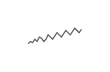
\begin{tikzpicture}[x=0.08em, y=0.08em, line width=0.4pt]
                \draw[FooterGray] (0,3) -- (1,4) -- (2,3.5) -- (3,5) -- (4,4) -- (5,6) -- (6,5.5) -- (7,4) -- (8,5) -- (9,7) -- (10,6) -- (11,5) -- (12,6.5) -- (13,8) -- (14,7) -- (15,6) -- (16,7.5) -- (17,9) -- (18,8) -- (19,7) -- (20,8.5) -- (21,10) -- (22,9) -- (23,8) -- (24,9.5);
            \end{tikzpicture}%
        }%
        \hskip0.5cm%
    }%
    \vskip6pt%
}

%=============================================================================
% PACKAGES
%=============================================================================
\usepackage[utf8]{inputenc}
\DeclareUnicodeCharacter{03B1}{\ensuremath{\alpha}}
\usepackage[T1]{fontenc}
\usepackage{amsmath, amssymb, amsthm}
\usepackage{mathtools}
\usepackage{bm}
\usepackage{tikz}
\usetikzlibrary{arrows.meta, positioning, shapes, calc, decorations.pathreplacing, shadings}
\usepackage{booktabs}
\usepackage{multirow}
\usepackage{array}
\usepackage{graphicx}
\usepackage{animate}
\usepackage{hyperref}
\usepackage{colortbl}
\usepackage{listings}
\lstset{language=Python, basicstyle=\ttfamily\scriptsize, keywordstyle=\color{MainBlue}\bfseries,
  commentstyle=\color{Forest}, stringstyle=\color{Crimson}, breaklines=true,
  frame=none, backgroundcolor=\color{VeryLightGray}, xleftmargin=2mm}
\hypersetup{colorlinks=true, linkcolor=MainBlue, urlcolor=MainBlue}
\graphicspath{{../../logos/}{../../charts/}{../../photos/}}
\usepackage{xcolor}
\hfuzz=2pt  % Suppress tiny overfull warnings (<2pt)
\vfuzz=2pt  % Suppress tiny vertical overfull warnings (<2pt)
% \mathrm in the sans-serif family of the slides (beamer resets \mathrm to the serif family at \begin{document};
% this hook runs after beamer's, so WN, Var, RMSE, ... in formulas match the surrounding text)
% Bold vectors and matrices in the same sans-serif family: \mathbf{A} in sans bold (beamer's own \mathbf came out in
% medium weight), and the bold upright Greek capitals of \boldsymbol / \bm (\bSigma, \bPhi, \boldsymbol{\Theta}) in
% cmss bold: bm.sty fixes its "boldoperators" font when it is loaded (serif cmbx), before beamer switches the
% operators to cmss, so it is reset here.
\AtBeginDocument{%
  \SetMathAlphabet{\mathrm}{normal}{\encodingdefault}{\sfdefault}{\mddefault}{n}%
  \SetMathAlphabet{\mathrm}{bold}{\encodingdefault}{\sfdefault}{bx}{n}%
  \SetMathAlphabet{\mathbf}{normal}{\encodingdefault}{\sfdefault}{bx}{n}%
  \SetMathAlphabet{\mathbf}{bold}{\encodingdefault}{\sfdefault}{bx}{n}%
  \SetSymbolFont{boldoperators}{normal}{OT1}{cmss}{bx}{n}%
  \SetSymbolFont{boldoperators}{bold}{OT1}{cmss}{bx}{n}}

%=============================================================================
% QUANTLET COMMANDS
%   \quantlet{<displayed name>}{<url>}       (generic, compatible with the older TSA decks)
%   \tsaquantlet{Ch_05}{TSA_ch5_garch}       -> https://github.com/danpele/Time-Series-Analysis/tree/main/Quantlets/Ch_05/TSA_ch5_garch
%   \qlurl{<folder>} is defined per chapter by the generator (Quantlets/Ch_NN/<folder>)
%=============================================================================
\newcommand{\tsarepo}{https://github.com/danpele/Time-Series-Analysis}
\newcommand{\tsaqlbase}{https://github.com/danpele/Time-Series-Analysis/tree/main/Quantlets}
\newcommand{\quantlet}[2]{%
    \hfill\href{#2}{%
        \raisebox{-0.15em}{
\includegraphics[height=0.7em]{ql_logo.png}}%
        \textcolor{MainBlue}{\tiny\ #1}%
    }%
}
\newcommand{\tsaquantlet}[2]{\quantlet{\detokenize{#2}}{\tsaqlbase/#1/#2}}

%=============================================================================
% NOTEBOOKS (Google Colab)
%   \colaburl{notebooks/EN/chapter5_seminar_notebook.ipynb} -> the Colab link of a file in the TSA repo
%   \nb: the chapter notebook (each seminar deck redefines it with \renewcommand)
%=============================================================================
\newcommand{\colaburl}[1]{https://colab.research.google.com/github/danpele/Time-Series-Analysis/blob/main/#1}
\newcommand{\nb}{https://colab.research.google.com/github/danpele/Time-Series-Analysis/tree/main/notebooks/EN}
\newcommand{\nbname}{notebooks/EN}

%=============================================================================
% SLIDE HELPERS (used by the generators; the same as in MFM)
%=============================================================================
% local font size for list bodies (the preamble forces \normalsize)
\newcommand{\itemsize}[1]{\setbeamertemplate{itemize/enumerate body begin}{#1}\setbeamertemplate{itemize/enumerate subbody begin}{#1}}
\newcommand{\intitle}[1]{{\hypersetup{urlcolor=white}#1}}   % white links inside coloured title bars
\newcommand{\imgcap}[1]{{\scriptsize #1}\\[0.5mm]}          % caption under a photo
\newcommand{\imgcredit}[2]{{\tiny\color{FooterGray}\href{#1}{#2}}}   % image credit: source URL, author/licence
\newcommand{\aiprompt}[1]{{\ttfamily\color{MainBlue}#1}}     % a prompt to an AI assistant

%=============================================================================
% SEMINARS: student version by default; the instructor wrapper *_solutions.tex sets \solutionstrue
%=============================================================================
\makeatletter\@ifundefined{ifsolutions}{\expandafter\newif\csname ifsolutions\endcsname}{}\makeatother
\newcommand{\solonly}[1]{\ifsolutions #1\fi}
\newcommand{\propsub}{\ifsolutions\else\framesubtitle{\ifdefined\tsalang Rezolvarea se discută la seminar\else Solution discussed in class\fi}\fi}

%=============================================================================
% APPENDIX AND CHAPTER LINKS (latex/appendix_links.py writes the calls; it also re-declares these
% macros before \begin{document}, so the decks compile with or without this preamble block)
%=============================================================================
\providecommand{\tsaapplink}[3]{\hypertarget{#2}{}\hyperlink{#1}{\beamergotobutton{#3}}}
\providecommand{\tsaappback}[2]{\begin{tikzpicture}[remember picture,overlay]\node[anchor=south east] at ([xshift=-3mm,yshift=7mm]current page.south east){\hyperlink{#1}{\beamerreturnbutton{#2}}};\end{tikzpicture}}
\providecommand{\tsachlink}[2]{\href{#1}{#2}}
\providecommand{\tsachlinkt}[2]{\href{#1}{\usebeamercolor[fg]{frametitle}#2}}

%=============================================================================
% QUANTINAR COMMAND: link către un curs Quantinar (subiecte avansate)
%=============================================================================
\newcommand{\quantinar}[2]{%
    \href{#2}{%
        \raisebox{-0.15em}{
\includegraphics[height=0.8em]{qr_logo.png}}%
        \textcolor{MainBlue}{\scriptsize\ #1}%
    }%
}

%=============================================================================
% CUSTOM TITLE PAGE
%=============================================================================
\defbeamertemplate*{title page}{hybrid}[1][]
{
    \vspace{0.2cm}
    % Logos row - top header (with clickable links)
    \begin{center}
        \href{https://www.ase.ro}{
\includegraphics[height=1.0cm]{ase_logo.png}}\hspace{0.3cm}%
        \href{https://theida.net}{
\includegraphics[height=1.0cm]{ida_logo.png}}\hspace{0.3cm}%
        \href{https://blockchain-research-center.com}{
\includegraphics[height=1.0cm]{brc_logo.png}}\hspace{0.3cm}%
        \href{https://www.ai4efin.ase.ro}{
\includegraphics[height=1.0cm]{ai4efin_logo.png}}\hspace{0.3cm}%
        \href{https://ipe.ro/new}{
\includegraphics[height=1.0cm]{acad_logo.png}}\hspace{0.3cm}%
        \href{https://www.digital-finance-msca.com}{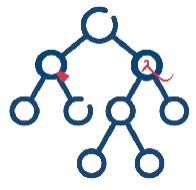
\includegraphics[height=1.0cm]{msca_logo.png}}%
    \end{center}

    \vspace{0.6cm}

    % Main title with Q logos on sides (with clickable links)
    \begin{center}
        \begin{minipage}{0.1\textwidth}
            \centering
            \href{https://quantlet.com}{
\includegraphics[height=1.1cm]{ql_logo.png}}
        \end{minipage}%
        \begin{minipage}{0.78\textwidth}
            \centering
            {\LARGE\bfseries\usebeamercolor[fg]{title}\inserttitle}

            \vspace{0.3cm}

            {\usebeamerfont{subtitle}\usebeamercolor[fg]{title}\insertsubtitle}
        \end{minipage}%
        \begin{minipage}{0.1\textwidth}
            \centering
            \href{https://quantinar.com}{
\includegraphics[height=1.1cm]{qr_logo.png}}
        \end{minipage}
    \end{center}

    \vspace{0.6cm}

    % Authors (left aligned)
    \hspace{0.5cm}{\usebeamerfont{author}\insertauthor}

    \vspace{0.3cm}

    % Institute/Affiliations (left aligned)
    \hspace{0.5cm}\begin{minipage}[t]{0.9\textwidth}
        \raggedright\small\insertinstitute
    \end{minipage}
}

%=============================================================================
% THEOREM ENVIRONMENTS
%=============================================================================
\theoremstyle{definition}
\setbeamertemplate{theorems}[numbered]
\ifdefined\tsalang
\newtheorem{defn}{Definiție}
\newtheorem{thm}{Teoremă}
\newtheorem{prop}{Propoziție}
\newtheorem{rmk}{Observație}
\else
\newtheorem{defn}{Definition}
\newtheorem{thm}{Theorem}
\newtheorem{prop}{Proposition}
\newtheorem{rmk}{Remark}
\fi

%=============================================================================
% CENTRED MINIPAGE (no extra vertical space)
%=============================================================================
\newenvironment{cminipage}[1]{%
    \par\noindent\hfill\begin{minipage}{#1}\ignorespaces
}{%
    \end{minipage}\hfill\null\par
}

%=============================================================================
% CUSTOM COMMANDS
%=============================================================================
\newcommand{\E}{\mathbb{E}}
\newcommand{\Var}{\text{Var}}
\newcommand{\Cov}{\text{Cov}}
\newcommand{\Corr}{\text{Corr}}
\newcommand{\R}{\mathbb{R}}
\newcommand{\N}{\mathbb{N}}
\newcommand{\Z}{\mathbb{Z}}
\newcommand{\B}{\mathbf{B}}
\newcommand{\imark}{\textcolor{MainBlue}{\textbullet}}
\newcommand{\RMSE}{\text{RMSE}}
\newcommand{\MAE}{\text{MAE}}
\newcommand{\MAPE}{\text{MAPE}}

% Boldface vector/matrix commands (VAR, VECM, state space; also used by the older TSA decks)
\newcommand{\bY}{\mathbf{Y}}
\newcommand{\bX}{\mathbf{X}}
\newcommand{\bA}{\mathbf{A}}
\newcommand{\bB}{\mathbf{B}}
\newcommand{\bepsilon}{\boldsymbol{\varepsilon}}
\newcommand{\bSigma}{\boldsymbol{\Sigma}}
\newcommand{\bPhi}{\boldsymbol{\Phi}}
\newcommand{\bGamma}{\boldsymbol{\Gamma}}
\newcommand{\bPi}{\boldsymbol{\Pi}}
\newcommand{\bc}{\mathbf{c}}
\newcommand{\balpha}{\boldsymbol{\alpha}}
\newcommand{\bbeta}{\boldsymbol{\beta}}
\newcommand{\bvarepsilon}{\boldsymbol{\varepsilon}}

% Legacy seminar marks (older TSA seminar decks)
\newcommand{\correct}{\textcolor{Forest}{\checkmark}}
\newcommand{\incorrect}{\textcolor{Crimson}{\texttimes}}
 se definește
%   \newcommand{\coursename}{Time Series Analysis}      (EN)
%   \newcommand{\coursename}{Serii de timp}       (RO)  și  \def\tsalang{ro}
% Fișierele .tex se află în EN/Courses, EN/Seminars, RO/Cursuri, RO/Seminarii (două niveluri sub rădăcină).
% Deck-urile sînt generate de latex/build_chapterN.py / build_seminarN.py (vezi latex/tsa_build.py).

\documentclass[9pt, aspectratio=169, t]{beamer}
\providecommand{\coursename}{Time Series Analysis}

% Ensure content fits on slides
\setbeamersize{text margin left=8mm, text margin right=8mm}
% Smaller institute font (title page)
\setbeamerfont{institute}{size=\footnotesize}

%=============================================================================
% THEME AND STYLE CONFIGURATION
%=============================================================================
\usetheme{default}
% Using default theme for clean header/footer control

% Color Palette (matching Redispatch PDF)
\definecolor{MainBlue}{RGB}{26, 58, 110}
\definecolor{AccentBlue}{RGB}{26, 58, 110}
\definecolor{IDAred}{RGB}{205, 0, 0}
\definecolor{DarkGray}{RGB}{51, 51, 51}
\definecolor{MediumGray}{RGB}{128, 128, 128}
\definecolor{LightGray}{RGB}{248, 248, 248}
\definecolor{VeryLightGray}{RGB}{235, 235, 235}
\definecolor{KeynoteGray}{RGB}{218, 218, 218}
\definecolor{SectionGray}{RGB}{120, 120, 120}
\definecolor{FooterGray}{RGB}{100, 100, 100}
\definecolor{Crimson}{RGB}{220, 53, 69}
\definecolor{Forest}{RGB}{46, 125, 50}
\definecolor{Amber}{RGB}{181, 133, 63}
\definecolor{Orange}{RGB}{230, 126, 34}
\definecolor{Purple}{RGB}{142, 68, 173}

% Gradient background (exact Keynote 315° gradient: white to RGB 218,218,218)
\setbeamertemplate{background}{%
    \begin{tikzpicture}[remember picture, overlay]
        \shade[shading=axis, shading angle=315,
        top color=white, bottom color=KeynoteGray]
        (current page.south west) rectangle (current page.north east);
    \end{tikzpicture}%
}
% Fallback solid color for compatibility
\setbeamercolor{background canvas}{bg=}

\setbeamercolor{palette primary}{bg=MainBlue, fg=white}
\setbeamercolor{palette secondary}{bg=MainBlue!85, fg=white}
\setbeamercolor{palette tertiary}{bg=MainBlue!70, fg=white}
\setbeamercolor{structure}{fg=MainBlue}
\setbeamercolor{title}{fg=IDAred}
\setbeamercolor{frametitle}{fg=IDAred, bg=}
\setbeamercolor{block title}{bg=MainBlue, fg=white}
\setbeamercolor{block body}{bg=VeryLightGray, fg=DarkGray}
\setbeamercolor{block title alerted}{bg=Crimson, fg=white}
\setbeamercolor{block body alerted}{bg=Crimson!8, fg=DarkGray}
\setbeamercolor{block title example}{bg=Forest, fg=white}
\setbeamercolor{block body example}{bg=Forest!8, fg=DarkGray}
\setbeamercolor{item}{fg=MainBlue}

% Footer colors (override Madrid theme blue)
\setbeamercolor{author in head/foot}{fg=FooterGray, bg=}
\setbeamercolor{title in head/foot}{fg=FooterGray, bg=}
\setbeamercolor{date in head/foot}{fg=FooterGray, bg=}
\setbeamercolor{section in head/foot}{fg=FooterGray, bg=}
\setbeamercolor{subsection in head/foot}{fg=FooterGray, bg=}

% Bullet styles (apply everywhere including blocks)
\setbeamertemplate{itemize item}{\color{MainBlue}$\boxdot$}
\setbeamertemplate{itemize subitem}{\color{MainBlue}$\blacktriangleright$}
\setbeamertemplate{itemize subsubitem}{\color{MainBlue}\tiny$\bullet$}
\setbeamertemplate{itemize/enumerate body begin}{\normalsize}
\setbeamertemplate{itemize/enumerate subbody begin}{\normalsize}

% Item spacing - compact style
\setlength{\leftmargini}{10pt}       % Level 1: minimal indent
\setlength{\leftmarginii}{10pt}      % Level 2: minimal additional indent
% Compact list spacing (zero extra space before/after lists in blocks)
\makeatletter
\def\@listi{\leftmargin\leftmargini \topsep 0pt \parsep 0pt \itemsep 0pt}
\def\@listii{\leftmargin\leftmarginii \topsep 0pt \parsep 0pt \itemsep 0pt}
\makeatother

\setbeamertemplate{navigation symbols}{}

%=============================================================================
% CUSTOM HEADLINE
%=============================================================================
\setbeamertemplate{headline}{%
    \vskip10pt%
    \hbox to \paperwidth{%
        \hskip0.5cm%
        {\small\color{FooterGray}\renewcommand{\hyperlink}[2]{##2}\insertsectionhead}%
        \hfill%
        \textcolor{FooterGray}{\small\insertframenumber}%
        \hskip0.5cm%
    }%
    \vskip4pt%
    {\color{FooterGray}\hrule height 0.4pt}%
}

%=============================================================================
% CUSTOM FOOTER
%=============================================================================
\usepackage{fontawesome5}

\setbeamertemplate{footline}{%
    {\color{FooterGray}\hrule height 0.4pt}%
    \vskip4pt%
    \hbox to \paperwidth{%
        \hskip0.5cm%
        \textcolor{FooterGray}{\small\coursename}%
        \hfill%
        \raisebox{-0.1em}{%
            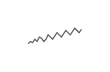
\begin{tikzpicture}[x=0.08em, y=0.08em, line width=0.4pt]
                \draw[FooterGray] (0,3) -- (1,4) -- (2,3.5) -- (3,5) -- (4,4) -- (5,6) -- (6,5.5) -- (7,4) -- (8,5) -- (9,7) -- (10,6) -- (11,5) -- (12,6.5) -- (13,8) -- (14,7) -- (15,6) -- (16,7.5) -- (17,9) -- (18,8) -- (19,7) -- (20,8.5) -- (21,10) -- (22,9) -- (23,8) -- (24,9.5);
            \end{tikzpicture}%
        }%
        \hskip0.5cm%
    }%
    \vskip6pt%
}

%=============================================================================
% PACKAGES
%=============================================================================
\usepackage[utf8]{inputenc}
\DeclareUnicodeCharacter{03B1}{\ensuremath{\alpha}}
\usepackage[T1]{fontenc}
\usepackage{amsmath, amssymb, amsthm}
\usepackage{mathtools}
\usepackage{bm}
\usepackage{tikz}
\usetikzlibrary{arrows.meta, positioning, shapes, calc, decorations.pathreplacing, shadings}
\usepackage{booktabs}
\usepackage{multirow}
\usepackage{array}
\usepackage{graphicx}
\usepackage{animate}
\usepackage{hyperref}
\usepackage{colortbl}
\usepackage{listings}
\lstset{language=Python, basicstyle=\ttfamily\scriptsize, keywordstyle=\color{MainBlue}\bfseries,
  commentstyle=\color{Forest}, stringstyle=\color{Crimson}, breaklines=true,
  frame=none, backgroundcolor=\color{VeryLightGray}, xleftmargin=2mm}
\hypersetup{colorlinks=true, linkcolor=MainBlue, urlcolor=MainBlue}
\graphicspath{{../../logos/}{../../charts/}{../../photos/}}
\usepackage{xcolor}
\hfuzz=2pt  % Suppress tiny overfull warnings (<2pt)
\vfuzz=2pt  % Suppress tiny vertical overfull warnings (<2pt)
% \mathrm in the sans-serif family of the slides (beamer resets \mathrm to the serif family at \begin{document};
% this hook runs after beamer's, so WN, Var, RMSE, ... in formulas match the surrounding text)
% Bold vectors and matrices in the same sans-serif family: \mathbf{A} in sans bold (beamer's own \mathbf came out in
% medium weight), and the bold upright Greek capitals of \boldsymbol / \bm (\bSigma, \bPhi, \boldsymbol{\Theta}) in
% cmss bold: bm.sty fixes its "boldoperators" font when it is loaded (serif cmbx), before beamer switches the
% operators to cmss, so it is reset here.
\AtBeginDocument{%
  \SetMathAlphabet{\mathrm}{normal}{\encodingdefault}{\sfdefault}{\mddefault}{n}%
  \SetMathAlphabet{\mathrm}{bold}{\encodingdefault}{\sfdefault}{bx}{n}%
  \SetMathAlphabet{\mathbf}{normal}{\encodingdefault}{\sfdefault}{bx}{n}%
  \SetMathAlphabet{\mathbf}{bold}{\encodingdefault}{\sfdefault}{bx}{n}%
  \SetSymbolFont{boldoperators}{normal}{OT1}{cmss}{bx}{n}%
  \SetSymbolFont{boldoperators}{bold}{OT1}{cmss}{bx}{n}}

%=============================================================================
% QUANTLET COMMANDS
%   \quantlet{<displayed name>}{<url>}       (generic, compatible with the older TSA decks)
%   \tsaquantlet{Ch_05}{TSA_ch5_garch}       -> https://github.com/danpele/Time-Series-Analysis/tree/main/Quantlets/Ch_05/TSA_ch5_garch
%   \qlurl{<folder>} is defined per chapter by the generator (Quantlets/Ch_NN/<folder>)
%=============================================================================
\newcommand{\tsarepo}{https://github.com/danpele/Time-Series-Analysis}
\newcommand{\tsaqlbase}{https://github.com/danpele/Time-Series-Analysis/tree/main/Quantlets}
\newcommand{\quantlet}[2]{%
    \hfill\href{#2}{%
        \raisebox{-0.15em}{
\includegraphics[height=0.7em]{ql_logo.png}}%
        \textcolor{MainBlue}{\tiny\ #1}%
    }%
}
\newcommand{\tsaquantlet}[2]{\quantlet{\detokenize{#2}}{\tsaqlbase/#1/#2}}

%=============================================================================
% NOTEBOOKS (Google Colab)
%   \colaburl{notebooks/EN/chapter5_seminar_notebook.ipynb} -> the Colab link of a file in the TSA repo
%   \nb: the chapter notebook (each seminar deck redefines it with \renewcommand)
%=============================================================================
\newcommand{\colaburl}[1]{https://colab.research.google.com/github/danpele/Time-Series-Analysis/blob/main/#1}
\newcommand{\nb}{https://colab.research.google.com/github/danpele/Time-Series-Analysis/tree/main/notebooks/EN}
\newcommand{\nbname}{notebooks/EN}

%=============================================================================
% SLIDE HELPERS (used by the generators; the same as in MFM)
%=============================================================================
% local font size for list bodies (the preamble forces \normalsize)
\newcommand{\itemsize}[1]{\setbeamertemplate{itemize/enumerate body begin}{#1}\setbeamertemplate{itemize/enumerate subbody begin}{#1}}
\newcommand{\intitle}[1]{{\hypersetup{urlcolor=white}#1}}   % white links inside coloured title bars
\newcommand{\imgcap}[1]{{\scriptsize #1}\\[0.5mm]}          % caption under a photo
\newcommand{\imgcredit}[2]{{\tiny\color{FooterGray}\href{#1}{#2}}}   % image credit: source URL, author/licence
\newcommand{\aiprompt}[1]{{\ttfamily\color{MainBlue}#1}}     % a prompt to an AI assistant

%=============================================================================
% SEMINARS: student version by default; the instructor wrapper *_solutions.tex sets \solutionstrue
%=============================================================================
\makeatletter\@ifundefined{ifsolutions}{\expandafter\newif\csname ifsolutions\endcsname}{}\makeatother
\newcommand{\solonly}[1]{\ifsolutions #1\fi}
\newcommand{\propsub}{\ifsolutions\else\framesubtitle{\ifdefined\tsalang Rezolvarea se discută la seminar\else Solution discussed in class\fi}\fi}

%=============================================================================
% APPENDIX AND CHAPTER LINKS (latex/appendix_links.py writes the calls; it also re-declares these
% macros before \begin{document}, so the decks compile with or without this preamble block)
%=============================================================================
\providecommand{\tsaapplink}[3]{\hypertarget{#2}{}\hyperlink{#1}{\beamergotobutton{#3}}}
\providecommand{\tsaappback}[2]{\begin{tikzpicture}[remember picture,overlay]\node[anchor=south east] at ([xshift=-3mm,yshift=7mm]current page.south east){\hyperlink{#1}{\beamerreturnbutton{#2}}};\end{tikzpicture}}
\providecommand{\tsachlink}[2]{\href{#1}{#2}}
\providecommand{\tsachlinkt}[2]{\href{#1}{\usebeamercolor[fg]{frametitle}#2}}

%=============================================================================
% QUANTINAR COMMAND: link către un curs Quantinar (subiecte avansate)
%=============================================================================
\newcommand{\quantinar}[2]{%
    \href{#2}{%
        \raisebox{-0.15em}{
\includegraphics[height=0.8em]{qr_logo.png}}%
        \textcolor{MainBlue}{\scriptsize\ #1}%
    }%
}

%=============================================================================
% CUSTOM TITLE PAGE
%=============================================================================
\defbeamertemplate*{title page}{hybrid}[1][]
{
    \vspace{0.2cm}
    % Logos row - top header (with clickable links)
    \begin{center}
        \href{https://www.ase.ro}{
\includegraphics[height=1.0cm]{ase_logo.png}}\hspace{0.3cm}%
        \href{https://theida.net}{
\includegraphics[height=1.0cm]{ida_logo.png}}\hspace{0.3cm}%
        \href{https://blockchain-research-center.com}{
\includegraphics[height=1.0cm]{brc_logo.png}}\hspace{0.3cm}%
        \href{https://www.ai4efin.ase.ro}{
\includegraphics[height=1.0cm]{ai4efin_logo.png}}\hspace{0.3cm}%
        \href{https://ipe.ro/new}{
\includegraphics[height=1.0cm]{acad_logo.png}}\hspace{0.3cm}%
        \href{https://www.digital-finance-msca.com}{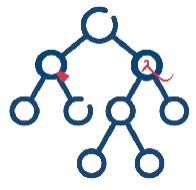
\includegraphics[height=1.0cm]{msca_logo.png}}%
    \end{center}

    \vspace{0.6cm}

    % Main title with Q logos on sides (with clickable links)
    \begin{center}
        \begin{minipage}{0.1\textwidth}
            \centering
            \href{https://quantlet.com}{
\includegraphics[height=1.1cm]{ql_logo.png}}
        \end{minipage}%
        \begin{minipage}{0.78\textwidth}
            \centering
            {\LARGE\bfseries\usebeamercolor[fg]{title}\inserttitle}

            \vspace{0.3cm}

            {\usebeamerfont{subtitle}\usebeamercolor[fg]{title}\insertsubtitle}
        \end{minipage}%
        \begin{minipage}{0.1\textwidth}
            \centering
            \href{https://quantinar.com}{
\includegraphics[height=1.1cm]{qr_logo.png}}
        \end{minipage}
    \end{center}

    \vspace{0.6cm}

    % Authors (left aligned)
    \hspace{0.5cm}{\usebeamerfont{author}\insertauthor}

    \vspace{0.3cm}

    % Institute/Affiliations (left aligned)
    \hspace{0.5cm}\begin{minipage}[t]{0.9\textwidth}
        \raggedright\small\insertinstitute
    \end{minipage}
}

%=============================================================================
% THEOREM ENVIRONMENTS
%=============================================================================
\theoremstyle{definition}
\setbeamertemplate{theorems}[numbered]
\ifdefined\tsalang
\newtheorem{defn}{Definiție}
\newtheorem{thm}{Teoremă}
\newtheorem{prop}{Propoziție}
\newtheorem{rmk}{Observație}
\else
\newtheorem{defn}{Definition}
\newtheorem{thm}{Theorem}
\newtheorem{prop}{Proposition}
\newtheorem{rmk}{Remark}
\fi

%=============================================================================
% CENTRED MINIPAGE (no extra vertical space)
%=============================================================================
\newenvironment{cminipage}[1]{%
    \par\noindent\hfill\begin{minipage}{#1}\ignorespaces
}{%
    \end{minipage}\hfill\null\par
}

%=============================================================================
% CUSTOM COMMANDS
%=============================================================================
\newcommand{\E}{\mathbb{E}}
\newcommand{\Var}{\text{Var}}
\newcommand{\Cov}{\text{Cov}}
\newcommand{\Corr}{\text{Corr}}
\newcommand{\R}{\mathbb{R}}
\newcommand{\N}{\mathbb{N}}
\newcommand{\Z}{\mathbb{Z}}
\newcommand{\B}{\mathbf{B}}
\newcommand{\imark}{\textcolor{MainBlue}{\textbullet}}
\newcommand{\RMSE}{\text{RMSE}}
\newcommand{\MAE}{\text{MAE}}
\newcommand{\MAPE}{\text{MAPE}}

% Boldface vector/matrix commands (VAR, VECM, state space; also used by the older TSA decks)
\newcommand{\bY}{\mathbf{Y}}
\newcommand{\bX}{\mathbf{X}}
\newcommand{\bA}{\mathbf{A}}
\newcommand{\bB}{\mathbf{B}}
\newcommand{\bepsilon}{\boldsymbol{\varepsilon}}
\newcommand{\bSigma}{\boldsymbol{\Sigma}}
\newcommand{\bPhi}{\boldsymbol{\Phi}}
\newcommand{\bGamma}{\boldsymbol{\Gamma}}
\newcommand{\bPi}{\boldsymbol{\Pi}}
\newcommand{\bc}{\mathbf{c}}
\newcommand{\balpha}{\boldsymbol{\alpha}}
\newcommand{\bbeta}{\boldsymbol{\beta}}
\newcommand{\bvarepsilon}{\boldsymbol{\varepsilon}}

% Legacy seminar marks (older TSA seminar decks)
\newcommand{\correct}{\textcolor{Forest}{\checkmark}}
\newcommand{\incorrect}{\textcolor{Crimson}{\texttimes}}
 se definește
%   \newcommand{\coursename}{Time Series Analysis}      (EN)
%   \newcommand{\coursename}{Serii de timp}       (RO)  și  \def\tsalang{ro}
% Fișierele .tex se află în EN/Courses, EN/Seminars, RO/Cursuri, RO/Seminarii (două niveluri sub rădăcină).
% Deck-urile sînt generate de latex/build_chapterN.py / build_seminarN.py (vezi latex/tsa_build.py).

\documentclass[9pt, aspectratio=169, t]{beamer}
\providecommand{\coursename}{Time Series Analysis}

% Ensure content fits on slides
\setbeamersize{text margin left=8mm, text margin right=8mm}
% Smaller institute font (title page)
\setbeamerfont{institute}{size=\footnotesize}

%=============================================================================
% THEME AND STYLE CONFIGURATION
%=============================================================================
\usetheme{default}
% Using default theme for clean header/footer control

% Color Palette (matching Redispatch PDF)
\definecolor{MainBlue}{RGB}{26, 58, 110}
\definecolor{AccentBlue}{RGB}{26, 58, 110}
\definecolor{IDAred}{RGB}{205, 0, 0}
\definecolor{DarkGray}{RGB}{51, 51, 51}
\definecolor{MediumGray}{RGB}{128, 128, 128}
\definecolor{LightGray}{RGB}{248, 248, 248}
\definecolor{VeryLightGray}{RGB}{235, 235, 235}
\definecolor{KeynoteGray}{RGB}{218, 218, 218}
\definecolor{SectionGray}{RGB}{120, 120, 120}
\definecolor{FooterGray}{RGB}{100, 100, 100}
\definecolor{Crimson}{RGB}{220, 53, 69}
\definecolor{Forest}{RGB}{46, 125, 50}
\definecolor{Amber}{RGB}{181, 133, 63}
\definecolor{Orange}{RGB}{230, 126, 34}
\definecolor{Purple}{RGB}{142, 68, 173}

% Gradient background (exact Keynote 315° gradient: white to RGB 218,218,218)
\setbeamertemplate{background}{%
    \begin{tikzpicture}[remember picture, overlay]
        \shade[shading=axis, shading angle=315,
        top color=white, bottom color=KeynoteGray]
        (current page.south west) rectangle (current page.north east);
    \end{tikzpicture}%
}
% Fallback solid color for compatibility
\setbeamercolor{background canvas}{bg=}

\setbeamercolor{palette primary}{bg=MainBlue, fg=white}
\setbeamercolor{palette secondary}{bg=MainBlue!85, fg=white}
\setbeamercolor{palette tertiary}{bg=MainBlue!70, fg=white}
\setbeamercolor{structure}{fg=MainBlue}
\setbeamercolor{title}{fg=IDAred}
\setbeamercolor{frametitle}{fg=IDAred, bg=}
\setbeamercolor{block title}{bg=MainBlue, fg=white}
\setbeamercolor{block body}{bg=VeryLightGray, fg=DarkGray}
\setbeamercolor{block title alerted}{bg=Crimson, fg=white}
\setbeamercolor{block body alerted}{bg=Crimson!8, fg=DarkGray}
\setbeamercolor{block title example}{bg=Forest, fg=white}
\setbeamercolor{block body example}{bg=Forest!8, fg=DarkGray}
\setbeamercolor{item}{fg=MainBlue}

% Footer colors (override Madrid theme blue)
\setbeamercolor{author in head/foot}{fg=FooterGray, bg=}
\setbeamercolor{title in head/foot}{fg=FooterGray, bg=}
\setbeamercolor{date in head/foot}{fg=FooterGray, bg=}
\setbeamercolor{section in head/foot}{fg=FooterGray, bg=}
\setbeamercolor{subsection in head/foot}{fg=FooterGray, bg=}

% Bullet styles (apply everywhere including blocks)
\setbeamertemplate{itemize item}{\color{MainBlue}$\boxdot$}
\setbeamertemplate{itemize subitem}{\color{MainBlue}$\blacktriangleright$}
\setbeamertemplate{itemize subsubitem}{\color{MainBlue}\tiny$\bullet$}
\setbeamertemplate{itemize/enumerate body begin}{\normalsize}
\setbeamertemplate{itemize/enumerate subbody begin}{\normalsize}

% Item spacing - compact style
\setlength{\leftmargini}{10pt}       % Level 1: minimal indent
\setlength{\leftmarginii}{10pt}      % Level 2: minimal additional indent
% Compact list spacing (zero extra space before/after lists in blocks)
\makeatletter
\def\@listi{\leftmargin\leftmargini \topsep 0pt \parsep 0pt \itemsep 0pt}
\def\@listii{\leftmargin\leftmarginii \topsep 0pt \parsep 0pt \itemsep 0pt}
\makeatother

\setbeamertemplate{navigation symbols}{}

%=============================================================================
% CUSTOM HEADLINE
%=============================================================================
\setbeamertemplate{headline}{%
    \vskip10pt%
    \hbox to \paperwidth{%
        \hskip0.5cm%
        {\small\color{FooterGray}\renewcommand{\hyperlink}[2]{##2}\insertsectionhead}%
        \hfill%
        \textcolor{FooterGray}{\small\insertframenumber}%
        \hskip0.5cm%
    }%
    \vskip4pt%
    {\color{FooterGray}\hrule height 0.4pt}%
}

%=============================================================================
% CUSTOM FOOTER
%=============================================================================
\usepackage{fontawesome5}

\setbeamertemplate{footline}{%
    {\color{FooterGray}\hrule height 0.4pt}%
    \vskip4pt%
    \hbox to \paperwidth{%
        \hskip0.5cm%
        \textcolor{FooterGray}{\small\coursename}%
        \hfill%
        \raisebox{-0.1em}{%
            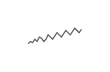
\begin{tikzpicture}[x=0.08em, y=0.08em, line width=0.4pt]
                \draw[FooterGray] (0,3) -- (1,4) -- (2,3.5) -- (3,5) -- (4,4) -- (5,6) -- (6,5.5) -- (7,4) -- (8,5) -- (9,7) -- (10,6) -- (11,5) -- (12,6.5) -- (13,8) -- (14,7) -- (15,6) -- (16,7.5) -- (17,9) -- (18,8) -- (19,7) -- (20,8.5) -- (21,10) -- (22,9) -- (23,8) -- (24,9.5);
            \end{tikzpicture}%
        }%
        \hskip0.5cm%
    }%
    \vskip6pt%
}

%=============================================================================
% PACKAGES
%=============================================================================
\usepackage[utf8]{inputenc}
\DeclareUnicodeCharacter{03B1}{\ensuremath{\alpha}}
\usepackage[T1]{fontenc}
\usepackage{amsmath, amssymb, amsthm}
\usepackage{mathtools}
\usepackage{bm}
\usepackage{tikz}
\usetikzlibrary{arrows.meta, positioning, shapes, calc, decorations.pathreplacing, shadings}
\usepackage{booktabs}
\usepackage{multirow}
\usepackage{array}
\usepackage{graphicx}
\usepackage{animate}
\usepackage{hyperref}
\usepackage{colortbl}
\usepackage{listings}
\lstset{language=Python, basicstyle=\ttfamily\scriptsize, keywordstyle=\color{MainBlue}\bfseries,
  commentstyle=\color{Forest}, stringstyle=\color{Crimson}, breaklines=true,
  frame=none, backgroundcolor=\color{VeryLightGray}, xleftmargin=2mm}
\hypersetup{colorlinks=true, linkcolor=MainBlue, urlcolor=MainBlue}
\graphicspath{{../../logos/}{../../charts/}{../../photos/}}
\usepackage{xcolor}
\hfuzz=2pt  % Suppress tiny overfull warnings (<2pt)
\vfuzz=2pt  % Suppress tiny vertical overfull warnings (<2pt)
% \mathrm in the sans-serif family of the slides (beamer resets \mathrm to the serif family at \begin{document};
% this hook runs after beamer's, so WN, Var, RMSE, ... in formulas match the surrounding text)
% Bold vectors and matrices in the same sans-serif family: \mathbf{A} in sans bold (beamer's own \mathbf came out in
% medium weight), and the bold upright Greek capitals of \boldsymbol / \bm (\bSigma, \bPhi, \boldsymbol{\Theta}) in
% cmss bold: bm.sty fixes its "boldoperators" font when it is loaded (serif cmbx), before beamer switches the
% operators to cmss, so it is reset here.
\AtBeginDocument{%
  \SetMathAlphabet{\mathrm}{normal}{\encodingdefault}{\sfdefault}{\mddefault}{n}%
  \SetMathAlphabet{\mathrm}{bold}{\encodingdefault}{\sfdefault}{bx}{n}%
  \SetMathAlphabet{\mathbf}{normal}{\encodingdefault}{\sfdefault}{bx}{n}%
  \SetMathAlphabet{\mathbf}{bold}{\encodingdefault}{\sfdefault}{bx}{n}%
  \SetSymbolFont{boldoperators}{normal}{OT1}{cmss}{bx}{n}%
  \SetSymbolFont{boldoperators}{bold}{OT1}{cmss}{bx}{n}}

%=============================================================================
% QUANTLET COMMANDS
%   \quantlet{<displayed name>}{<url>}       (generic, compatible with the older TSA decks)
%   \tsaquantlet{Ch_05}{TSA_ch5_garch}       -> https://github.com/danpele/Time-Series-Analysis/tree/main/Quantlets/Ch_05/TSA_ch5_garch
%   \qlurl{<folder>} is defined per chapter by the generator (Quantlets/Ch_NN/<folder>)
%=============================================================================
\newcommand{\tsarepo}{https://github.com/danpele/Time-Series-Analysis}
\newcommand{\tsaqlbase}{https://github.com/danpele/Time-Series-Analysis/tree/main/Quantlets}
\newcommand{\quantlet}[2]{%
    \hfill\href{#2}{%
        \raisebox{-0.15em}{
\includegraphics[height=0.7em]{ql_logo.png}}%
        \textcolor{MainBlue}{\tiny\ #1}%
    }%
}
\newcommand{\tsaquantlet}[2]{\quantlet{\detokenize{#2}}{\tsaqlbase/#1/#2}}

%=============================================================================
% NOTEBOOKS (Google Colab)
%   \colaburl{notebooks/EN/chapter5_seminar_notebook.ipynb} -> the Colab link of a file in the TSA repo
%   \nb: the chapter notebook (each seminar deck redefines it with \renewcommand)
%=============================================================================
\newcommand{\colaburl}[1]{https://colab.research.google.com/github/danpele/Time-Series-Analysis/blob/main/#1}
\newcommand{\nb}{https://colab.research.google.com/github/danpele/Time-Series-Analysis/tree/main/notebooks/EN}
\newcommand{\nbname}{notebooks/EN}

%=============================================================================
% SLIDE HELPERS (used by the generators; the same as in MFM)
%=============================================================================
% local font size for list bodies (the preamble forces \normalsize)
\newcommand{\itemsize}[1]{\setbeamertemplate{itemize/enumerate body begin}{#1}\setbeamertemplate{itemize/enumerate subbody begin}{#1}}
\newcommand{\intitle}[1]{{\hypersetup{urlcolor=white}#1}}   % white links inside coloured title bars
\newcommand{\imgcap}[1]{{\scriptsize #1}\\[0.5mm]}          % caption under a photo
\newcommand{\imgcredit}[2]{{\tiny\color{FooterGray}\href{#1}{#2}}}   % image credit: source URL, author/licence
\newcommand{\aiprompt}[1]{{\ttfamily\color{MainBlue}#1}}     % a prompt to an AI assistant

%=============================================================================
% SEMINARS: student version by default; the instructor wrapper *_solutions.tex sets \solutionstrue
%=============================================================================
\makeatletter\@ifundefined{ifsolutions}{\expandafter\newif\csname ifsolutions\endcsname}{}\makeatother
\newcommand{\solonly}[1]{\ifsolutions #1\fi}
\newcommand{\propsub}{\ifsolutions\else\framesubtitle{\ifdefined\tsalang Rezolvarea se discută la seminar\else Solution discussed in class\fi}\fi}

%=============================================================================
% APPENDIX AND CHAPTER LINKS (latex/appendix_links.py writes the calls; it also re-declares these
% macros before \begin{document}, so the decks compile with or without this preamble block)
%=============================================================================
\providecommand{\tsaapplink}[3]{\hypertarget{#2}{}\hyperlink{#1}{\beamergotobutton{#3}}}
\providecommand{\tsaappback}[2]{\begin{tikzpicture}[remember picture,overlay]\node[anchor=south east] at ([xshift=-3mm,yshift=7mm]current page.south east){\hyperlink{#1}{\beamerreturnbutton{#2}}};\end{tikzpicture}}
\providecommand{\tsachlink}[2]{\href{#1}{#2}}
\providecommand{\tsachlinkt}[2]{\href{#1}{\usebeamercolor[fg]{frametitle}#2}}

%=============================================================================
% QUANTINAR COMMAND: link către un curs Quantinar (subiecte avansate)
%=============================================================================
\newcommand{\quantinar}[2]{%
    \href{#2}{%
        \raisebox{-0.15em}{
\includegraphics[height=0.8em]{qr_logo.png}}%
        \textcolor{MainBlue}{\scriptsize\ #1}%
    }%
}

%=============================================================================
% CUSTOM TITLE PAGE
%=============================================================================
\defbeamertemplate*{title page}{hybrid}[1][]
{
    \vspace{0.2cm}
    % Logos row - top header (with clickable links)
    \begin{center}
        \href{https://www.ase.ro}{
\includegraphics[height=1.0cm]{ase_logo.png}}\hspace{0.3cm}%
        \href{https://theida.net}{
\includegraphics[height=1.0cm]{ida_logo.png}}\hspace{0.3cm}%
        \href{https://blockchain-research-center.com}{
\includegraphics[height=1.0cm]{brc_logo.png}}\hspace{0.3cm}%
        \href{https://www.ai4efin.ase.ro}{
\includegraphics[height=1.0cm]{ai4efin_logo.png}}\hspace{0.3cm}%
        \href{https://ipe.ro/new}{
\includegraphics[height=1.0cm]{acad_logo.png}}\hspace{0.3cm}%
        \href{https://www.digital-finance-msca.com}{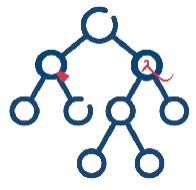
\includegraphics[height=1.0cm]{msca_logo.png}}%
    \end{center}

    \vspace{0.6cm}

    % Main title with Q logos on sides (with clickable links)
    \begin{center}
        \begin{minipage}{0.1\textwidth}
            \centering
            \href{https://quantlet.com}{
\includegraphics[height=1.1cm]{ql_logo.png}}
        \end{minipage}%
        \begin{minipage}{0.78\textwidth}
            \centering
            {\LARGE\bfseries\usebeamercolor[fg]{title}\inserttitle}

            \vspace{0.3cm}

            {\usebeamerfont{subtitle}\usebeamercolor[fg]{title}\insertsubtitle}
        \end{minipage}%
        \begin{minipage}{0.1\textwidth}
            \centering
            \href{https://quantinar.com}{
\includegraphics[height=1.1cm]{qr_logo.png}}
        \end{minipage}
    \end{center}

    \vspace{0.6cm}

    % Authors (left aligned)
    \hspace{0.5cm}{\usebeamerfont{author}\insertauthor}

    \vspace{0.3cm}

    % Institute/Affiliations (left aligned)
    \hspace{0.5cm}\begin{minipage}[t]{0.9\textwidth}
        \raggedright\small\insertinstitute
    \end{minipage}
}

%=============================================================================
% THEOREM ENVIRONMENTS
%=============================================================================
\theoremstyle{definition}
\setbeamertemplate{theorems}[numbered]
\ifdefined\tsalang
\newtheorem{defn}{Definiție}
\newtheorem{thm}{Teoremă}
\newtheorem{prop}{Propoziție}
\newtheorem{rmk}{Observație}
\else
\newtheorem{defn}{Definition}
\newtheorem{thm}{Theorem}
\newtheorem{prop}{Proposition}
\newtheorem{rmk}{Remark}
\fi

%=============================================================================
% CENTRED MINIPAGE (no extra vertical space)
%=============================================================================
\newenvironment{cminipage}[1]{%
    \par\noindent\hfill\begin{minipage}{#1}\ignorespaces
}{%
    \end{minipage}\hfill\null\par
}

%=============================================================================
% CUSTOM COMMANDS
%=============================================================================
\newcommand{\E}{\mathbb{E}}
\newcommand{\Var}{\text{Var}}
\newcommand{\Cov}{\text{Cov}}
\newcommand{\Corr}{\text{Corr}}
\newcommand{\R}{\mathbb{R}}
\newcommand{\N}{\mathbb{N}}
\newcommand{\Z}{\mathbb{Z}}
\newcommand{\B}{\mathbf{B}}
\newcommand{\imark}{\textcolor{MainBlue}{\textbullet}}
\newcommand{\RMSE}{\text{RMSE}}
\newcommand{\MAE}{\text{MAE}}
\newcommand{\MAPE}{\text{MAPE}}

% Boldface vector/matrix commands (VAR, VECM, state space; also used by the older TSA decks)
\newcommand{\bY}{\mathbf{Y}}
\newcommand{\bX}{\mathbf{X}}
\newcommand{\bA}{\mathbf{A}}
\newcommand{\bB}{\mathbf{B}}
\newcommand{\bepsilon}{\boldsymbol{\varepsilon}}
\newcommand{\bSigma}{\boldsymbol{\Sigma}}
\newcommand{\bPhi}{\boldsymbol{\Phi}}
\newcommand{\bGamma}{\boldsymbol{\Gamma}}
\newcommand{\bPi}{\boldsymbol{\Pi}}
\newcommand{\bc}{\mathbf{c}}
\newcommand{\balpha}{\boldsymbol{\alpha}}
\newcommand{\bbeta}{\boldsymbol{\beta}}
\newcommand{\bvarepsilon}{\boldsymbol{\varepsilon}}

% Legacy seminar marks (older TSA seminar decks)
\newcommand{\correct}{\textcolor{Forest}{\checkmark}}
\newcommand{\incorrect}{\textcolor{Crimson}{\texttimes}}


\newcommand{\qlurl}[1]{https://github.com/danpele/Time-Series-Analysis/tree/main/Quantlets/Ch_12/#1}

% Clickable citations (DOIs verified via Crossref)
\newcommand{\refHP}{\href{https://doi.org/10.1007/978-3-031-13584-2}{Huang și Petukhina (2022)}}
\newcommand{\refSS}{\href{https://doi.org/10.1007/978-3-319-52452-8}{Shumway și Stoffer (2017)}}
\newcommand{\refBDtm}{\href{https://doi.org/10.1007/978-1-4419-0320-4}{Brockwell și Davis (1991)}}
\newcommand{\refHamTS}{\href{https://doi.org/10.1515/9780691218632}{Hamilton (1994)}}
\newcommand{\refSchuster}{\href{https://doi.org/10.1029/TM003i001p00013}{Schuster (1898)}}
\newcommand{\refYule}{\href{https://doi.org/10.1098/rsta.1927.0007}{Yule (1927)}}
\newcommand{\refFisher}{\href{https://doi.org/10.1098/rspa.1929.0151}{Fisher (1929)}}
\newcommand{\refBartlett}{\href{https://doi.org/10.1093/biomet/37.1-2.1}{Bartlett (1950)}}
\newcommand{\refBT}{\href{https://doi.org/10.1002/j.1538-7305.1958.tb03874.x}{Blackman și Tukey (1958)}}
\newcommand{\refCT}{\href{https://doi.org/10.1090/S0025-5718-1965-0178586-1}{Cooley și Tukey (1965)}}
\newcommand{\refGranger}{\href{https://doi.org/10.2307/1909859}{Granger (1966)}}
\newcommand{\refWelch}{\href{https://doi.org/10.1109/TAU.1967.1161901}{Welch (1967)}}
\newcommand{\refGPH}{\href{https://doi.org/10.1111/j.1467-9892.1983.tb00371.x}{Geweke și Porter-Hudak (1983)}}
\newcommand{\refHPf}{\href{https://doi.org/10.2307/2953682}{Hodrick și Prescott (1997)}}
\newcommand{\refTC}{\href{https://doi.org/10.1175/1520-0477(1998)079<0061:APGTWA>2.0.CO;2}{Torrence și Compo (1998)}}
\newcommand{\refBK}{\href{https://doi.org/10.1162/003465399558454}{Baxter și King (1999)}}
\newcommand{\refHamHP}{\href{https://doi.org/10.1162/rest_a_00706}{Hamilton (2018)}}

\title[Serii de timp]{Serii de timp}
\subtitle{Capitolul 12: Analiză spectrală}
\author[D.T. Pele]{Daniel Traian PELE}
\institute{Academia de Studii Economice din București\\
IDA Institute Digital Assets\\
Blockchain Research Center\\
AI4EFin Artificial Intelligence for Energy Finance\\
Academia Română, Institutul de Prognoză Economică\\
MSCA Digital Finance}
\date{}

%=============================================================================
\providecommand{\tsaapplink}[3]{\hypertarget{#2}{}\hyperlink{#1}{\beamergotobutton{#3}}}  % APPLINKS-MACROS
\providecommand{\tsaappback}[2]{\begin{tikzpicture}[remember picture,overlay]\node[anchor=south east] at ([xshift=-3mm,yshift=7mm]current page.south east){\hyperlink{#1}{\beamerreturnbutton{#2}}};\end{tikzpicture}}  % APPLINKS-MACROS
\providecommand{\tsachlink}[2]{\href{#1}{#2}}  % APPLINKS-MACROS
\providecommand{\tsachlinkt}[2]{\href{#1}{\usebeamercolor[fg]{frametitle}#2}}  % APPLINKS-MACROS
\begin{document}
%=============================================================================

{
\setbeamertemplate{headline}{}
\setbeamertemplate{footline}{}
\begin{frame}[noframenumbering]
    \titlepage
\end{frame}
}
% BEGIN-ACRONYMS (generat de latex/acronyms.py; nu editati manual)
\begin{frame}{Acronime folosite în acest material}
\setbeamertemplate{itemize/enumerate body begin}{\tiny}
\begin{columns}[T]
\begin{column}{0.49\textwidth}
\begin{itemize}\setlength{\itemsep}{0pt}
    \item \textbf{ACF}: Autocorrelation Function (funcția de autocorelație)
    \item \textbf{AI}: Artificial Intelligence (inteligență artificială)
    \item \textbf{AR}: AutoRegressive (model); in event studies: Abnormal Return (model autoregresiv; în studiile de eveniment: randament anormal)
    \item \textbf{ARFIMA}: AutoRegressive Fractionally Integrated Moving Average (model) — model autoregresiv fracționar integrat cu medie mobilă
    \item \textbf{ARMA}: AutoRegressive Moving Average (model) — model autoregresiv cu medie mobilă
    \item \textbf{CWT}: Continuous Wavelet Transform (transformata wavelet continuă)
    \item \textbf{DFT}: Discrete Fourier Transform (transformata Fourier discretă)
    \item \textbf{ENTSO-E}: European Network of Transmission System Operators for Electricity (rețeaua europeană a operatorilor de transport și de sistem pentru energie electrică)
    \item \textbf{EODHD}: EOD Historical Data (market-data provider) — furnizor de date de piață
    \item \textbf{FFT}: Fast Fourier Transform (transformata Fourier rapidă)
    \item \textbf{FRED}: Federal Reserve Economic Data (baza de date economice a Rezervei Federale din St. Louis)
    \item \textbf{GDPC1}: Real Gross Domestic Product, chained dollars (FRED series code) — codul FRED al PIB-ului real al SUA
    \item \textbf{GPH}: Geweke–Porter-Hudak (estimator) — estimatorul Geweke–Porter-Hudak al parametrului de memorie lungă
\end{itemize}
\end{column}
\begin{column}{0.49\textwidth}
\begin{itemize}\setlength{\itemsep}{0pt}
    \item \textbf{HP}: Hodrick–Prescott (filter) — filtrul Hodrick–Prescott
    \item \textbf{INDPRO}: Industrial Production Index (FRED series code) — codul FRED al indicelui producției industriale din SUA
    \item \textbf{LPPL}: Log-Periodic Power Law (legea de putere log-periodică)
    \item \textbf{MA}: Moving Average (medie mobilă)
    \item \textbf{MW}: Megawatt (megawatt)
    \item \textbf{OLS}: Ordinary Least Squares (metoda celor mai mici pătrate)
    \item \textbf{PIB}: Produsul intern brut
    \item \textbf{SILSO}: Sunspot Index and Long-term Solar Observations (centrul mondial de date pentru numărul de pete solare (Observatorul Regal al Belgiei))
    \item \textbf{STFT}: Short-Time Fourier Transform (transformata Fourier pe ferestre scurte)
    \item \textbf{SUA}: Statele Unite ale Americii
    \item \textbf{UE}: Uniunea Europeană
    \item \textbf{UNRATE}: Unemployment Rate (FRED series code) — codul FRED al ratei șomajului din SUA
    \item \textbf{UTC}: Coordinated Universal Time (Temps Universel Coordonné) — timpul universal coordonat
\end{itemize}
\end{column}
\end{columns}
\end{frame}
% END-ACRONYMS

\begin{frame}{Întrebarea capitolului și traseul}
\itemsize{\small}
\begin{itemize}
    \item \textbf{Întrebarea}: ce cicluri conține o serie și cît din varianța ei explică fiecare ciclu?
    \begin{itemize}
        \item exemple: ciclul de 11 ani al petelor solare, ciclul economic, ritmul zilnic și săptămînal al consumului de energie electrică
    \end{itemize}
    \item \textbf{Traseul} capitolului
    \begin{itemize}
        \item cicluri, frecvențe și transformata Fourier discretă
        \item densitatea spectrală a zgomotului alb și a modelelor ARMA
        \item periodograma, slăbiciunile ei și netezirea ei
        \item cicluri în date; memoria lungă; filtre; două serii; o trimitere spre wavelets
    \end{itemize}
    \item Capitol de studiu individual: exemple rezolvate, slide-uri de interpretare și o recapitulare după fiecare secțiune; autoevaluare cu răspunsuri la final
\end{itemize}
\end{frame}

\begin{frame}{Rezultatele învățării}
\itemsize{\small}
\begin{itemize}
    \item Treceți de la frecvență la perioadă și la frecvența unghiulară și găsiți frecvențele Fourier ale unui eșantion
    \item Calculați densitatea spectrală a zgomotului alb și a modelelor AR(1), MA(1) și AR(2) și interpretați forma ei
    \item Calculați de mînă periodograma unei serii scurte și explicați de ce periodograma brută nu este consistentă
    \item Netezați periodograma (Daniell, Bartlett, Welch), aplicați o fereastră de atenuare și construiți benzi de încredere chi-pătrat
    \item Identificați cicluri în petele solare, în PIB și în consumul de energie electrică; interpretați coerența și faza dintre două serii
\end{itemize}
\end{frame}

\begin{frame}{Bibliografie și instrumente}
\itemsize{\small}
\begin{itemize}
    \item Referința principală a capitolului: \refSS, \tsachlink{https://danpele.github.io/Time-Series-Analysis/RO/Cursuri/capitol4_sezonalitate_prognoza.pdf}{capitolul 4} (analiză spectrală și filtrare)
    \begin{itemize}
        \item teorie: \refBDtm, \tsachlink{https://danpele.github.io/Time-Series-Analysis/RO/Cursuri/capitol4_sezonalitate_prognoza.pdf}{capitolele 4} și \tsachlink{https://danpele.github.io/Time-Series-Analysis/RO/Cursuri/capitol10_spatiul_starilor_kalman_markov_switching.pdf}{10}; \refHamTS, \tsachlink{https://danpele.github.io/Time-Series-Analysis/RO/Cursuri/capitol6_modele_var_cauzalitate_granger.pdf}{capitolul 6}; aplicații în Python: \refHP
        \item \refSS\ măsoară frecvența în cicluri pe observație; în \tsachlink{https://danpele.github.io/Time-Series-Analysis/RO/Cursuri/capitol8_memorie_lunga_arfima.pdf}{Capitolul 8} am folosit frecvența unghiulară $\lambda = 2\pi\nu$
    \end{itemize}
    \item Quantlet-urile Python ale capitolului: \href{https://github.com/danpele/Time-Series-Analysis/tree/main/Quantlets/Ch_12}{Quantlets/Ch\_12}
    \begin{itemize}
        \item periodograma, netezirea Daniell și wavelet-ul Morlet sînt scrise explicit în \texttt{numpy}; Welch și coerența provin din \texttt{scipy.signal}
    \end{itemize}
    \item Notebook-ul cursului: \href{\colaburl{notebooks/EN/chapter12_lecture_notebook.ipynb}}{deschideți în Google Colab}
    \item Curs video: \quantinar{Applied Time Series Analysis with Python}{https://quantinar.com/course/137/applied-time-series-analysis-with-python}
\end{itemize}
\end{frame}


%=============================================================================
\section{Cicluri și frecvențe}
%=============================================================================

\begin{frame}{Joseph Fourier și ideea capitolului}
\itemsize{\small}
\begin{columns}[T]
\begin{column}{0.36\textwidth}
\centering
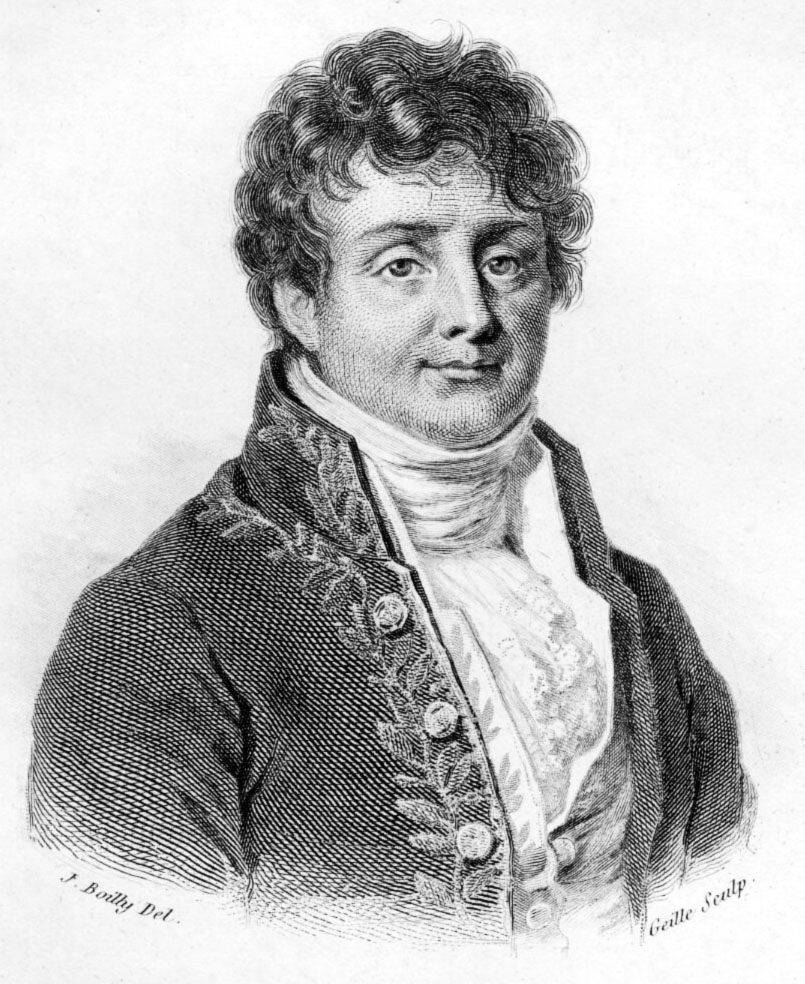
\includegraphics[height=0.5\textheight]{ch12_joseph_fourier.jpg}\\[1mm]
\imgcap{J. B. J. Fourier (1768--1830)}
\imgcredit{https://commons.wikimedia.org/wiki/File:Joseph_Fourier.jpg}{Gravură: A. F. B. Geille, după J.-L. Boilly (1839--1840); domeniu public; Wikimedia Commons}
\end{column}
\begin{column}{0.62\textwidth}
\begin{itemize}
    \item Fourier (1807, conducția căldurii): o funcție se poate scrie ca sumă de sinusuri și cosinusuri
    \begin{itemize}
        \item fiecare termen este un ciclu pur, cu frecvența și amplitudinea lui
    \end{itemize}
    \item Aplicat unei serii de timp: cîtă varianță se află la fiecare frecvență?
    \begin{itemize}
        \item \textbf{domeniul timpului} (\tsachlink{https://danpele.github.io/Time-Series-Analysis/RO/Cursuri/capitol1_procese_stochastice_stationaritate.pdf}{Capitolele 1}--\tsachlink{https://danpele.github.io/Time-Series-Analysis/RO/Cursuri/capitol8_memorie_lunga_arfima.pdf}{8}) descrie seria prin autocorelațiile ei
        \item \textbf{domeniul frecvenței} descrie aceeași informație prin spectru
    \end{itemize}
    \item Cele două perspective sînt echivalente; spectrul face ciclurile vizibile dintr-o privire
\end{itemize}
\end{column}
\end{columns}
\end{frame}

\begin{frame}{Un ciclu: amplitudine, frecvență, fază}
\itemsize{\small}
\begin{itemize}
    \item Un ciclu pur: $x_t = A\cos(2\pi\nu t + \varphi)$, $t = 1, 2, \ldots$
    \begin{itemize}
        \item $A$: \textbf{amplitudinea} (înălțimea undei); $\varphi$: \textbf{faza} (punctul de pornire al undei)
        \item $\nu$: \textbf{frecvența}, în cicluri pe observație; \textbf{perioada} $1/\nu$ este numărul de observații dintr-un ciclu
        \item frecvența unghiulară $\omega = 2\pi\nu$, în radiani pe observație
    \end{itemize}
    \item Exemplu: date lunare cu un ciclu anual: $\nu = 1/12$ cicluri pe lună, perioada 12 luni
    \begin{itemize}
        \item date orare cu un ciclu zilnic: $\nu = 1/24$; date trimestriale cu un ciclu de 6 ani: tot $\nu = 1/24$
    \end{itemize}
    \item Forma echivalentă: $A\cos(2\pi\nu t + \varphi) = a\cos(2\pi\nu t) + b\sin(2\pi\nu t)$
    \begin{itemize}
        \item cu $a = A\cos\varphi$, $b = -A\sin\varphi$ și $A^2 = a^2 + b^2$: liniară în $a$ și $b$, deci se poate estima prin OLS
    \end{itemize}
    \item Cea mai mare frecvență vizibilă în date discrete este $\nu = 1/2$ (un ciclu la două observații): \textbf{frecvența Nyquist}
\end{itemize}
\end{frame}

\begin{frame}{Două cicluri plus zgomot}
\itemsize{\footnotesize}
\begin{center}
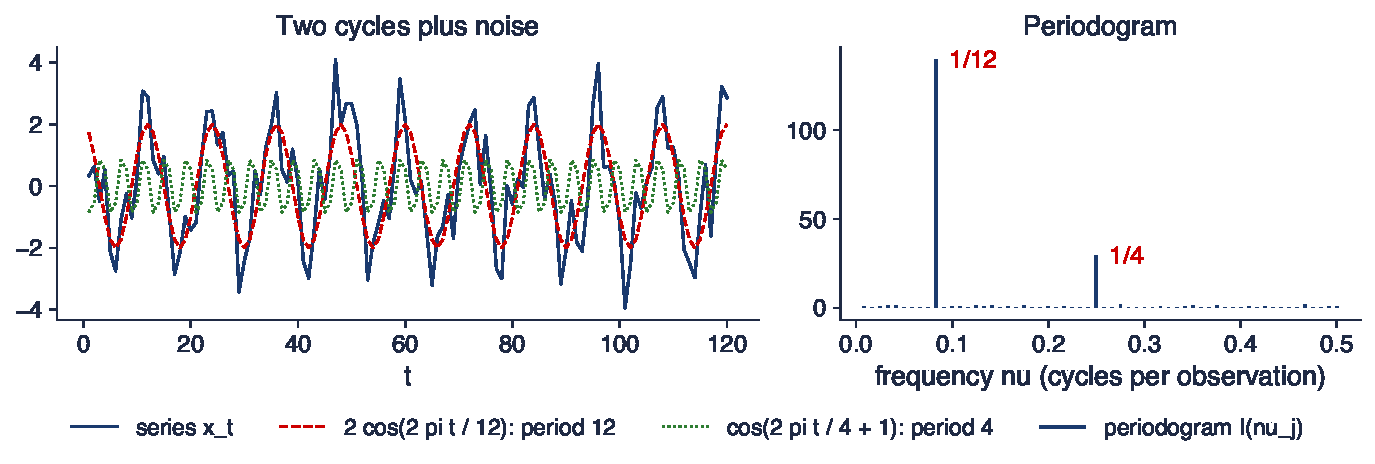
\includegraphics[width=0.97\textwidth,height=0.62\textheight,keepaspectratio]{tsa_ch12_fourier.pdf}
\end{center}
\vspace{-0.25cm}
\begin{itemize}
    \item Serie simulată, $T = 120$: $x_t = 2\cos(2\pi t/12) + \cos(2\pi t/4 + 1) + \varepsilon_t$, $\varepsilon_t \sim N(0;\ 0{,}49)$ (zgomot alb Normal cu varianța 0,49); dreapta: periodograma ei (definită în secțiunea 3)
\end{itemize}
\quantlet{TSA\_ch12\_fourier}{\qlurl{TSA_ch12_fourier}}
\end{frame}

\begin{frame}{Interpretarea celor două cicluri plus zgomot}
\itemsize{\small}
\begin{itemize}
    \item În domeniul timpului cele două cicluri sînt greu de separat cu ochiul liber
    \begin{itemize}
        \item în domeniul frecvenței ele sînt două vîrfuri izolate, la $\nu = 1/12$ și $\nu = 1/4$
    \end{itemize}
    \item Înălțimea vîrfurilor: 139{,}7 și 29{,}6; teoria, pentru un ciclu de amplitudine $A$ la o frecvență Fourier: $A^2T/4$, adică 120 și 30
    \begin{itemize}
        \item vîrful crește cu pătratul amplitudinii: ciclul mai mare domină
    \end{itemize}
    \item Cele două vîrfuri concentrează 85\% din puterea totală; zgomotul împrăștie restul uniform pe toate frecvențele
\end{itemize}
\end{frame}

\begin{frame}{Frecvențele Fourier și transformata Fourier discretă (1/2)}
\itemsize{\small}
\begin{itemize}
    \item Pentru un eșantion $x_1, \ldots, x_T$, \textbf{frecvențele Fourier} sînt $\nu_j = j/T$, $j = 0, 1, \ldots, \lfloor T/2 \rfloor$
    \begin{itemize}
        \item ciclurile care încap de un număr întreg de ori ($j$ ori) în eșantion; $\lfloor T/2 \rfloor$: partea întreagă a lui $T/2$
    \end{itemize}
    \item \textbf{Transformata Fourier discretă} (DFT) măsoară cît de puternic se mișcă seria împreună cu un ciclu de frecvență $\nu_j$
    \begin{itemize}
        \item $d(\nu_j) = T^{-1/2}\sum_{t=1}^{T} x_t\, e^{-2\pi i \nu_j t}$
        \item $i$: unitatea imaginară, $i^2 = -1$; $e^{-i\theta} = \cos\theta - i\sin\theta$ (formula lui Euler)
        \item deci DFT corelează seria cu un cosinus (partea reală) și cu un sinus (partea imaginară) de frecvență $\nu_j$
    \end{itemize}
\end{itemize}
\end{frame}

\begin{frame}{Frecvențele Fourier și transformata Fourier discretă (2/2)}
\itemsize{\small}
\begin{itemize}
    \item Cele $T$ valori $d(\nu_j)$ conțin exact aceeași informație ca cele $T$ observații
    \begin{itemize}
        \item datele se pot reconstitui din ele prin transformata inversă
    \end{itemize}
    \item \textbf{Parseval}
    \begin{itemize}
        \item suma pătratelor abaterilor este egală cu suma pătratelor modulelor DFT
        \item $\sum_{t=1}^{T}(x_t - \bar x)^2 = \sum_{j=1}^{T-1}|d(\nu_j)|^2$
        \item $\bar x$: media de selecție; $|d|^2 = (\mathrm{Re}\,d)^2 + (\mathrm{Im}\,d)^2$: pătratul modulului unui număr complex
        \item interpretarea: varianța seriei se împarte pe frecvențe
    \end{itemize}
    \item \textbf{Transformata Fourier rapidă} (FFT) a lui \refCT\ calculează rapid toate valorile $d(\nu_j)$
    \begin{itemize}
        \item $O(T\log T)$ operații în loc de $O(T^2)$: numărul de operații crește ca $T\log T$, nu ca $T^2$
    \end{itemize}
\end{itemize}
\end{frame}

\begin{frame}{Exemplu rezolvat: DFT pentru patru numere}
\itemsize{\small}
\begin{itemize}
    \item Datele: $x = (4, 2, 0, 2)$, $T = 4$; media $\bar x = 2$, abaterile $y = (2, 0, -2, 0)$
    \begin{itemize}
        \item Frecvențele Fourier: $\nu_1 = 1/4$ (perioada 4) și $\nu_2 = 1/2$ (perioada 2)
    \end{itemize}
    \item La $\nu = 1/4$: $e^{-2\pi i t/4} = e^{-i\pi t/2}$ este $-i$ pentru $t = 1$ și $i$ pentru $t = 3$
    \begin{itemize}
        \item $\sum_t y_t e^{-i\pi t/2} = 2(-i) + (-2)(i) = -4i$, deci $d(1/4) = -4i/\sqrt{4} = -2i$ și $|d(1/4)|^2 = 4$
    \end{itemize}
    \item La $\nu = 1/2$: $e^{-i\pi t} = (-1)^t$, deci $\sum_t y_t(-1)^t = -2 + 2 = 0$ și $|d(1/2)|^2 = 0$
    \begin{itemize}
        \item prin simetrie $|d(3/4)|^2 = |d(1/4)|^2 = 4$
    \end{itemize}
    \item Parseval: $4 + 0 + 4 = 8 = 2^2 + 0^2 + (-2)^2 + 0^2$; toată varianța ($8/4 = 2$) se află la perioada 4
    \item Verificare în Python: \texttt{abs(np.fft.fft([2, 0, -2, 0]))**2 / 4} dă $(0, 4, 0, 4)$
\end{itemize}
\end{frame}

\begin{frame}{Aliasing}
\itemsize{\footnotesize}
\begin{center}
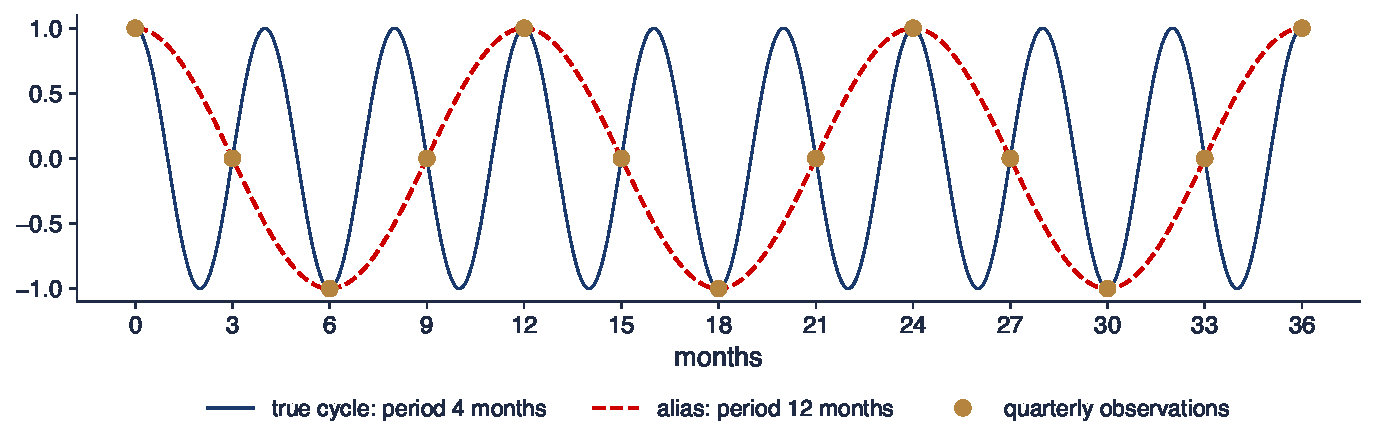
\includegraphics[width=0.97\textwidth,height=0.6\textheight,keepaspectratio]{tsa_ch12_aliasing.pdf}
\end{center}
\vspace{-0.25cm}
\begin{itemize}
    \item Un ciclu de 4 luni ($\nu = 1/4$ pe lună), observat doar o dată pe trimestru (la fiecare 3 luni)
\end{itemize}
\quantlet{TSA\_ch12\_aliasing}{\qlurl{TSA_ch12_aliasing}}
\end{frame}

\begin{frame}{Interpretarea fenomenului de aliasing}
\itemsize{\small}
\begin{itemize}
    \item Pe trimestru, frecvența adevărată este $3 \times 1/4 = 3/4$ cicluri, peste frecvența Nyquist $1/2$
    \begin{itemize}
        \item ea se pliază înapoi la $|3/4 - 1| = 1/4$ cicluri pe trimestru: o perioadă de 4 trimestre, adică 12 luni
    \end{itemize}
    \item Punctele trimestriale cad exact pe o undă de 12 luni: datele nu pot deosebi cele două cicluri
    \begin{itemize}
        \item acesta este \textbf{aliasing}: ciclurile mai rapide decît două observații apar ca cicluri mai lente, false
    \end{itemize}
    \item Regula practică: eșantionați de cel puțin două ori pe ciclul de interes; la agregarea pe o frecvență mai mică, faceți media valorilor, nu alegeți una dintre ele
\end{itemize}
\end{frame}

\begin{frame}{Recapitulare: cicluri și frecvențe}
\itemsize{\small}
\begin{itemize}
    \item Un ciclu are o amplitudine, o frecvență $\nu$ (cicluri pe observație), o perioadă $1/\nu$ și o fază
    \item DFT la frecvențele Fourier $j/T$ rescrie datele ca sumă de cicluri; Parseval împarte varianța pe frecvențe
    \item Sînt vizibile doar frecvențele pînă la $1/2$; ciclurile mai rapide apar ca aliasuri
\end{itemize}
\end{frame}


%=============================================================================
\section{Densitatea spectrală}
%=============================================================================

\begin{frame}{De la autocovarianțe la spectru}
\itemsize{\footnotesize}
\begin{itemize}
    \item Pentru o serie staționară cu autocovarianțele $\gamma(h)$, $\sum_h|\gamma(h)| < \infty$, \textbf{densitatea spectrală} este
    \begin{itemize}
        \item $f(\nu) = \sum_{h=-\infty}^{\infty}\gamma(h)e^{-2\pi i\nu h} = \gamma(0) + 2\sum_{h=1}^{\infty}\gamma(h)\cos(2\pi\nu h)$, $-1/2 \le \nu \le 1/2$
        \item $\gamma(h) = \mathrm{Cov}(x_t, x_{t+h})$: autocovarianța la lagul $h$; $\sum_h|\gamma(h)| < \infty$: autocovarianțele se sting suficient de repede (memorie scurtă)
        \item în cuvinte: $f(\nu)$ este o sumă ponderată a autocovarianțelor, cu ponderile $\cos(2\pi\nu h)$, care oscilează cu frecvența $\nu$
    \end{itemize}
    \item Relația inversă: $\gamma(h) = \int_{-1/2}^{1/2} f(\nu)e^{2\pi i\nu h}\,d\nu$
    \begin{itemize}
        \item perechea $\gamma \leftrightarrow f$ este teorema \textbf{Wiener--Khinchin}: autocovarianțele și spectrul conțin aceeași informație
        \item pentru $h = 0$: $\mathrm{Var}(x_t) = \gamma(0) = \int_{-1/2}^{1/2} f(\nu)\,d\nu$: aria de sub $f$ este varianța
    \end{itemize}
    \item Proprietăți: $f(\nu) \ge 0$, $f(-\nu) = f(\nu)$; este suficient să desenăm $f$ pe $[0, 1/2]$
    \begin{itemize}
        \item $f(\nu)\,d\nu$ este partea din varianță datorată ciclurilor cu frecvențe în $[\nu, \nu + d\nu]$
    \end{itemize}
\end{itemize}
\end{frame}

\begin{frame}{Zgomot alb, AR(1) și MA(1)}
\itemsize{\footnotesize}
\begin{itemize}
    \item \textbf{Zgomot alb} $w_t$, cu varianța $\sigma^2$
    \begin{itemize}
        \item $\gamma(h) = 0$ pentru $h \ne 0$, deci $f(\nu) = \sigma^2$ pentru orice $\nu$
        \item un spectru plat: toate frecvențele contribuie în mod egal, ca lumina albă
    \end{itemize}
    \item \textbf{AR(1)} $x_t = \phi x_{t-1} + w_t$, $|\phi| < 1$
    \begin{itemize}
        \item $f(\nu) = \dfrac{\sigma^2}{1 - 2\phi\cos(2\pi\nu) + \phi^2}$
        \item $\phi$: coeficientul autoregresiv; $w_t$: zgomot alb cu varianța $\sigma^2$
        \item $\phi > 0$: putere la frecvențele joase (serie netedă, persistentă); $\phi < 0$: putere la frecvențele înalte (serie în zigzag)
    \end{itemize}
    \item \textbf{MA(1)} $x_t = w_t + \theta w_{t-1}$
    \begin{itemize}
        \item $f(\nu) = \sigma^2\,[1 + 2\theta\cos(2\pi\nu) + \theta^2]$
        \item $\theta$: coeficientul de medie mobilă; $\theta > 0$ pune puterea la frecvențele joase, $\theta < 0$ la cele înalte
        \item direct din definiție: $\gamma(0) = \sigma^2(1 + \theta^2)$, $\gamma(1) = \sigma^2\theta$, deci $f = \gamma(0) + 2\gamma(1)\cos(2\pi\nu)$
    \end{itemize}
\end{itemize}
\end{frame}

\begin{frame}{Spectrul unui model ARMA}
\itemsize{\small}
\begin{itemize}
    \item \textbf{ARMA}$(p,q)$
    \begin{itemize}
        \item $\phi(L)x_t = \theta(L)w_t$
        \item $L$: operatorul lag, $Lx_t = x_{t-1}$
        \item $\phi(z) = 1 - \phi_1 z - \cdots - \phi_p z^p$ și $\theta(z) = 1 + \theta_1 z + \cdots + \theta_q z^q$: polinoamele AR și MA
    \end{itemize}
    \item Densitatea spectrală: cele două polinoame evaluate în $z = e^{-2\pi i\nu}$
    \begin{itemize}
        \item $f(\nu) = \sigma^2\dfrac{|\theta(e^{-2\pi i\nu})|^2}{|\phi(e^{-2\pi i\nu})|^2}$
        \item partea MA (numărătorul) adaugă putere acolo unde $|\theta|$ este mare; partea AR (numitorul) adaugă putere acolo unde $|\phi|$ este mic
    \end{itemize}
    \item Un raport de două polinoame în $\cos(2\pi\nu)$: neted și ușor de calculat (\refBDtm, secț.~4.4)
\end{itemize}
\end{frame}

\begin{frame}{Exemplu rezolvat: spectrele AR(1) și MA(1)}
\itemsize{\small}
\begin{itemize}
    \item AR(1) cu $\phi = 0{,}6$, $\sigma^2 = 1$
    \begin{itemize}
        \item $\nu = 0$: $\cos 0 = 1$, $f(0) = 1/(1 - 0{,}6)^2 = 1/0{,}16 = 6{,}25$
        \item $\nu = 1/2$: $\cos\pi = -1$, $f(1/2) = 1/(1 + 0{,}6)^2 = 1/2{,}56 = 0{,}39$
        \item raportul 16: ciclurile lente poartă mult mai multă varianță decît cele rapide
    \end{itemize}
    \item MA(1) cu $\theta = 0{,}5$, $\sigma^2 = 1$
    \begin{itemize}
        \item $f(0) = (1 + 0{,}5)^2 = 2{,}25$ și $f(1/2) = (1 - 0{,}5)^2 = 0{,}25$
    \end{itemize}
    \item Verificarea ariei pentru AR(1): $\int_{-1/2}^{1/2} f = \gamma(0) = 1/(1 - \phi^2) = 1/0{,}64 = 1{,}5625$
    \begin{itemize}
        \item integrala numerică a formulei dă aceeași valoare
    \end{itemize}
\end{itemize}
\end{frame}

\begin{frame}{AR(2) și pseudo-ciclurile}
\itemsize{\small}
\begin{itemize}
    \item \textbf{AR(2)} $x_t = \phi_1 x_{t-1} + \phi_2 x_{t-2} + w_t$
    \begin{itemize}
        \item $f(\nu) = \dfrac{\sigma^2}{|1 - \phi_1 e^{-2\pi i\nu} - \phi_2 e^{-4\pi i\nu}|^2}$
        \item pentru rădăcini complexe ($\phi_1^2 + 4\phi_2 < 0$) ACF este o undă amortizată, iar spectrul are un vîrf în interiorul intervalului $(0, 1/2)$
        \item vîrful se află la frecvența $\nu^*$ dată de $\cos(2\pi\nu^*) = \phi_1(\phi_2 - 1)/(4\phi_2)$, cînd membrul drept este în $[-1, 1]$
    \end{itemize}
    \item Un \textbf{pseudo-ciclu}
    \begin{itemize}
        \item un ciclu neregulat, a cărui lungime și amplitudine variază de la o rundă la alta
        \item \refYule\ a estimat un AR(2) pentru numerele de pete solare ale lui Wolfer: primul model autoregresiv, o alternativă la undele sinusoidale fixe
    \end{itemize}
    \item Ciclurile economice sînt pseudo-cicluri de acest fel: recurente, dar niciodată de aceeași lungime (secțiunea 5)
\end{itemize}
\end{frame}

\begin{frame}{Exemplu rezolvat: vîrful spectrului unui AR(2)}
\itemsize{\small}
\begin{itemize}
    \item $\phi_1 = 1{,}5$, $\phi_2 = -0{,}75$, $\sigma^2 = 1$; rădăcini complexe, deoarece $1{,}5^2 + 4(-0{,}75) = -0{,}75 < 0$
    \begin{itemize}
        \item $\cos(2\pi\nu^*) = 1{,}5 \cdot (-1{,}75)/(-3) = 0{,}875$, deci $\nu^* = \arccos(0{,}875)/(2\pi) = 0{,}0804$
        \item perioada $1/\nu^* = 12{,}4$ observații; pentru date anuale, un ciclu de aproximativ 12 ani
    \end{itemize}
    \item Înălțimea: $f(\nu^*) = 64$, față de $f(0) = 1/(1 - 1{,}5 + 0{,}75)^2 = 16$
    \begin{itemize}
        \item un vîrf clar: seria oscilează cu o perioadă tipică de aproximativ 12 observații
    \end{itemize}
    \item Același AR(2) este folosit în secțiunea 4 pentru a testa estimatorii spectrului
\end{itemize}
\end{frame}

\begin{frame}{O galerie de densități spectrale}
\itemsize{\footnotesize}
\begin{center}
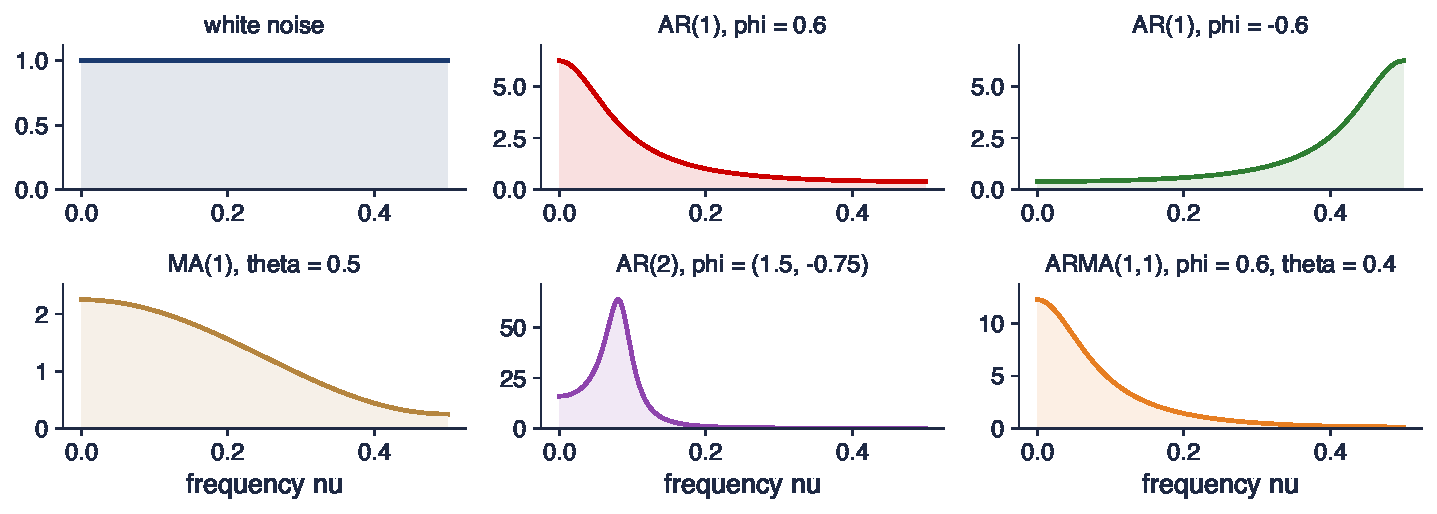
\includegraphics[width=0.97\textwidth,height=0.66\textheight,keepaspectratio]{tsa_ch12_spectra.pdf}
\end{center}
\vspace{-0.25cm}
\begin{itemize}
    \item Spectre teoretice, cu $\sigma^2 = 1$, pe $0 \le \nu \le 1/2$; aria hașurată este jumătate din varianță
\end{itemize}
\quantlet{TSA\_ch12\_spectra}{\qlurl{TSA_ch12_spectra}}
\end{frame}

\begin{frame}{Interpretarea galeriei}
\itemsize{\small}
\begin{itemize}
    \item Locul în care se află puterea arată tipul de dependență
    \begin{itemize}
        \item plat: nicio dependență (zgomot alb); descrescător: persistență pozitivă (AR(1) cu $\phi > 0$, MA(1) cu $\theta > 0$, ARMA(1,1))
        \item crescător: alternanță de semne (AR(1) cu $\phi < 0$); o cocoașă în interiorul benzii: un pseudo-ciclu (AR(2))
    \end{itemize}
    \item AR(2) își concentrează varianța 8{,}62 într-o bandă îngustă în jurul lui $\nu = 0{,}0804$
    \begin{itemize}
        \item ARMA(1,1) adaugă termenul MA la AR(1): $f(0) = 12{,}25$, o scădere mai abruptă
    \end{itemize}
    \item Ordinea de lucru: estimați spectrul din date, priviți forma lui, apoi alegeți un model care are un spectru asemănător
\end{itemize}
\end{frame}

\begin{frame}{Recapitulare: densitatea spectrală}
\itemsize{\small}
\begin{itemize}
    \item $f(\nu) = \sum_h\gamma(h)e^{-2\pi i\nu h}$; aria de sub $f$ este varianța; $f$ și ACF sînt echivalente
    \item Zgomotul alb are spectrul plat; AR(1) cu $\phi > 0$ pune puterea la frecvențele joase; AR(2) cu rădăcini complexe dă un vîrf
    \item Spectrele ARMA: $\sigma^2|\theta(e^{-2\pi i\nu})|^2/|\phi(e^{-2\pi i\nu})|^2$
\end{itemize}
\end{frame}


%=============================================================================
\section{Periodograma}
%=============================================================================

\begin{frame}{Arthur Schuster și periodicitățile ascunse}
\itemsize{\small}
\begin{columns}[T]
\begin{column}{0.36\textwidth}
\centering
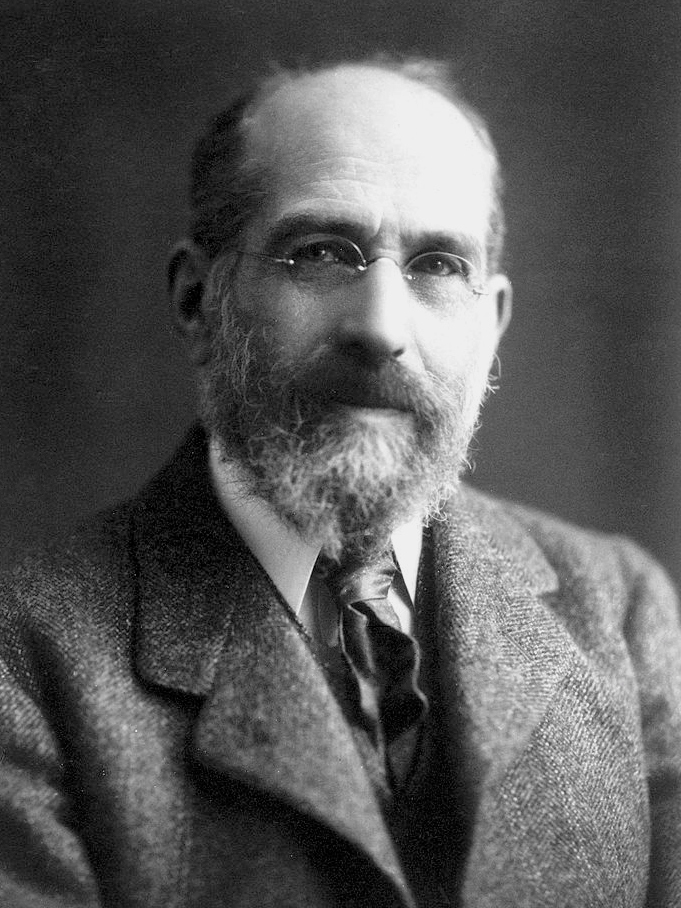
\includegraphics[height=0.5\textheight]{ch12_arthur_schuster.jpg}\\[1mm]
\imgcap{A. Schuster (1851--1934)}
\imgcredit{https://commons.wikimedia.org/wiki/File:Arthur_Schuster.jpg}{Foto: autor necunoscut (1900s); domeniu public; Wikimedia Commons}
\end{column}
\begin{column}{0.62\textwidth}
\begin{itemize}
    \item \refSchuster\ a introdus \textbf{periodograma} pentru a căuta „periodicități ascunse” în date meteorologice
    \begin{itemize}
        \item un presupus ciclu de 26 de zile; a arătat cum se judecă dacă un vîrf poate fi întîmplător
    \end{itemize}
    \item Petele solare: numărate zilnic încă din secolul al XVIII-lea; Rudolf Wolf a construit indicele standard în 1848
    \begin{itemize}
        \item ciclul lor de 11 ani este cazul clasic de test al analizei spectrale (\tsachlink{https://danpele.github.io/Time-Series-Analysis/RO/Cursuri/capitol0_introducere.pdf}{Capitolul 0})
    \end{itemize}
    \item Întrebarea secțiunii: cum estimăm $f(\nu)$ dintr-un singur eșantion și cît de sigură este estimarea?
\end{itemize}
\end{column}
\end{columns}
\end{frame}

\begin{frame}{Periodograma}
\itemsize{\small}
\begin{itemize}
    \item \textbf{Periodograma}
    \begin{itemize}
        \item $I(\nu_j) = |d(\nu_j)|^2$ la frecvențele Fourier $\nu_j = j/T$ (după eliminarea mediei)
        \item echivalent $I(\nu_j) = \sum_{|h| < T}\hat\gamma(h)e^{-2\pi i\nu_j h}$: formula spectrului cu autocovarianțele de selecție $\hat\gamma(h)$
    \end{itemize}
    \item Interpretarea prin regresie: regresați $x_t$ pe $\cos(2\pi\nu_j t)$ și $\sin(2\pi\nu_j t)$ prin OLS, cu coeficienții $a_j, b_j$
    \begin{itemize}
        \item $I(\nu_j) = \frac{T}{4}(a_j^2 + b_j^2)$: pătratul amplitudinii celui mai bun ciclu la $\nu_j$, înmulțit cu $T/4$
    \end{itemize}
    \item Descompunerea varianței: $\hat\gamma(0) = \frac{1}{T}\sum_{j=1}^{T-1} I(\nu_j)$
    \begin{itemize}
        \item ponderea unei benzi de frecvențe este suma ordonatelor ei împărțită la total
    \end{itemize}
    \item În Python: \texttt{np.abs(np.fft.fft(x - x.mean()))**2 / T}; se păstrează $j = 1, \ldots, \lfloor T/2\rfloor$
\end{itemize}
\end{frame}

\begin{frame}{Petele solare și periodograma lor}
\itemsize{\footnotesize}
\begin{center}
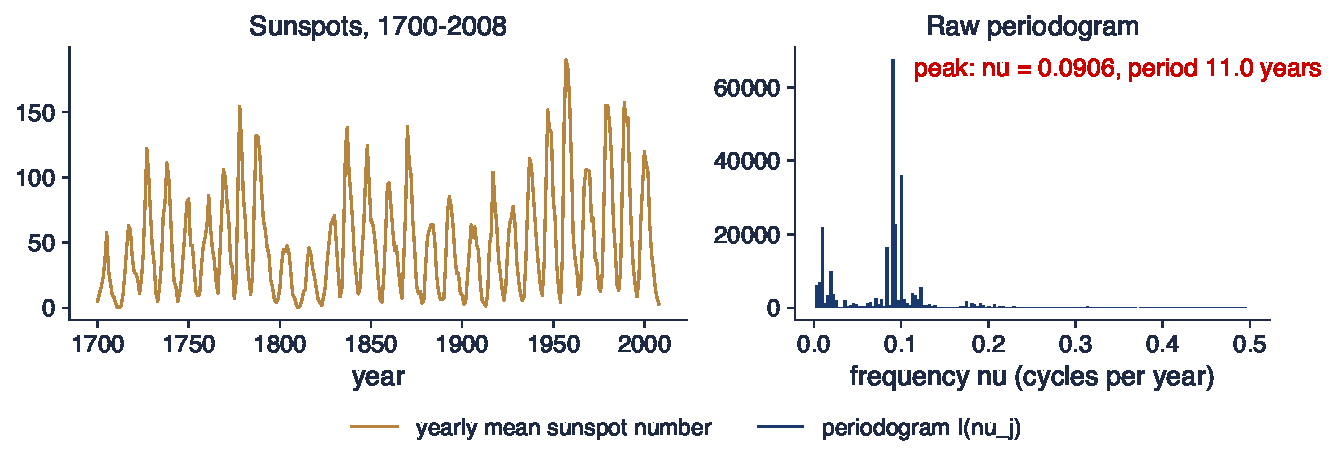
\includegraphics[width=0.97\textwidth,height=0.62\textheight,keepaspectratio]{tsa_ch12_sunspots.pdf}
\end{center}
\vspace{-0.25cm}
\begin{itemize}
    \item Numărul mediu anual de pete solare, 1700--2008, 309 observații (seria Wolf / SILSO, statsmodels); dreapta: periodograma brută
\end{itemize}
\quantlet{TSA\_ch12\_sunspots}{\qlurl{TSA_ch12_sunspots}}
\end{frame}

\begin{frame}{Interpretarea periodogramei petelor solare}
\itemsize{\small}
\begin{itemize}
    \item Cea mai mare ordonată este la $j = 28$: $\nu = 28/309 = 0{,}0906$ cicluri pe an, o perioadă de 11{,}0 ani
    \begin{itemize}
        \item următoarele ordonate ca mărime sînt la 10{,}0 și 10{,}7 ani: ciclul nu este perfect regulat
    \end{itemize}
    \item Perioadele între 9 și 13 ani explică 60\% din varianță
    \begin{itemize}
        \item ordonatele mici din apropierea lui $\nu = 0$ reflectă schimbările lente ale înălțimii ciclurilor (de exemplu ciclurile slabe din jurul anului 1800)
    \end{itemize}
    \item Periodograma brută este foarte zimțată: ordonatele vecine sar în sus și în jos; slide-urile următoare explică de ce
\end{itemize}
\end{frame}

\begin{frame}{Proprietățile statistice ale periodogramei}
\itemsize{\footnotesize}
\begin{itemize}
    \item Pentru $T$ mare, la o frecvență Fourier $0 < \nu_j < 1/2$ (\refBDtm, secț.~10.3; \refSS, secț.~4.3):
    \begin{itemize}
        \item $\dfrac{2I(\nu_j)}{f(\nu_j)} \approx \chi^2_2$: deci $E[I(\nu_j)] \approx f(\nu_j)$ (nedeplasată) și $\mathrm{Var}[I(\nu_j)] \approx f(\nu_j)^2$
        \item $\chi^2_2$: distribuția chi-pătrat cu 2 grade de libertate (media 2, varianța 4); $f(\nu_j)$: densitatea spectrală adevărată
        \item ordonatele de la frecvențe Fourier diferite sînt aproximativ independente
    \end{itemize}
    \item Varianța \textbf{nu} scade cînd $T$ crește
    \begin{itemize}
        \item periodograma \textbf{nu este un estimator consistent} al lui $f$
        \item un $T$ mai mare dă mai multe ordonate (o grilă mai fină), nu ordonate mai precise
    \end{itemize}
    \item $\chi^2_2/2$ este o distribuție exponențială cu media 1: o singură ordonată poate depăși ușor de 3 ori valoarea adevărată
    \begin{itemize}
        \item cuantila ei de 95\% este 3{,}00: aproximativ 1 ordonată din 20 depășește întîmplător $3{,}00\,f(\nu)$
    \end{itemize}
\end{itemize}
\end{frame}

\begin{frame}{Periodograma zgomotului alb}
\itemsize{\footnotesize}
\begin{center}
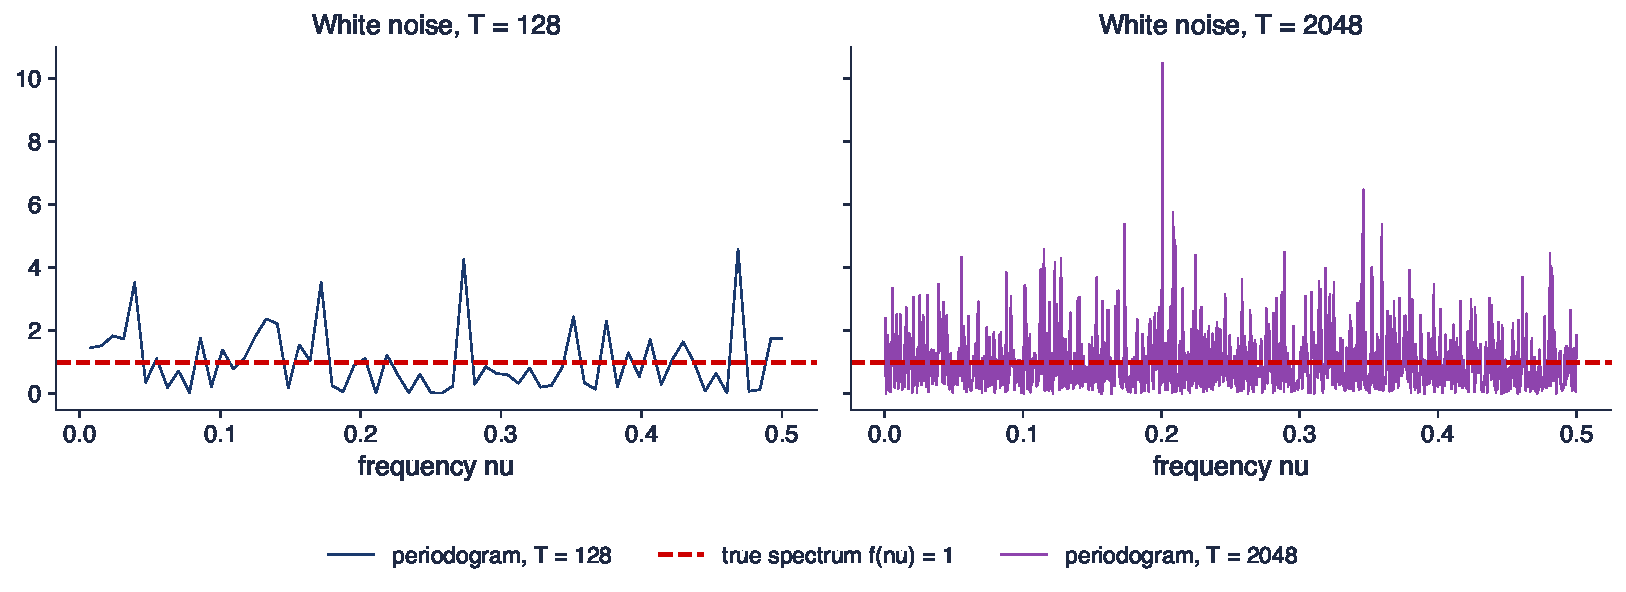
\includegraphics[width=0.97\textwidth,height=0.6\textheight,keepaspectratio]{tsa_ch12_inconsistency.pdf}
\end{center}
\vspace{-0.25cm}
\begin{itemize}
    \item Zgomot alb gaussian cu $\sigma^2 = 1$, deci spectrul adevărat este constant, egal cu 1; eșantioane de $T = 128$ și $T = 2048$
\end{itemize}
\quantlet{TSA\_ch12\_inconsistency}{\qlurl{TSA_ch12_inconsistency}}
\end{frame}

\begin{frame}{Interpretarea periodogramei zgomotului alb}
\itemsize{\small}
\begin{itemize}
    \item $T = 128$: media ordonatelor 1{,}03, abaterea standard 1{,}03
    \begin{itemize}
        \item $T = 2048$: media 1{,}01, abaterea standard 1{,}00: de 16 ori mai multe date, aceeași împrăștiere
    \end{itemize}
    \item Cea mai mare ordonată pentru $T = 2048$ este 10{,}5: din 1024 de ordonate, apar întîmplător vîrfuri înalte izolate
    \begin{itemize}
        \item un vîrf înalt nu este încă un ciclu: are nevoie de un test (slide-ul următor) sau de o estimare netezită (secțiunea 4)
    \end{itemize}
    \item Media este corectă (aproximativ 1): periodograma este nedeplasată, dar zgomotoasă; media ordonatelor vecine va reduce zgomotul
\end{itemize}
\end{frame}

\begin{frame}{Testul lui Fisher pentru o periodicitate ascunsă (1/2)}
\itemsize{\small}
\begin{itemize}
    \item Ipotezele
    \begin{itemize}
        \item $H_0$: zgomot alb gaussian; $H_1$: zgomot alb plus un ciclu la o frecvență Fourier necunoscută
    \end{itemize}
    \item Statistica lui \refFisher: ponderea celei mai mari ordonate în suma tuturor ordonatelor
    \begin{itemize}
        \item $g = \max_j I(\nu_j)\,/\,\sum_{j=1}^{m} I(\nu_j)$
        \item $m$: numărul de ordonate din $(0, 1/2)$; $\max_j$: cea mai mare dintre ele; $1/m \le g \le 1$
    \end{itemize}
    \item Interpretarea
    \begin{itemize}
        \item sub $H_0$ fiecare ordonată reprezintă aproximativ $1/m$ din total
        \item un $g$ mult mai mare decît $1/m$ semnalează un ciclu: o singură frecvență preia o parte mare din varianță
    \end{itemize}
\end{itemize}
\end{frame}

\begin{frame}{Testul lui Fisher pentru o periodicitate ascunsă (2/2)}
\itemsize{\small}
\begin{itemize}
    \item P-value-ul exact: probabilitatea, sub $H_0$, ca $g$ să depășească valoarea observată $x$
    \begin{itemize}
        \item $P(g > x) = \sum_{k \ge 1,\ kx < 1}(-1)^{k-1}\binom{m}{k}(1 - kx)^{m-1}$
        \item $k$: indicele de însumare, de la 1 cît timp $kx < 1$; $\binom{m}{k}$: coeficientul binomial
        \item un p-value mic (sub 0,05): se respinge zgomotul alb în favoarea unui ciclu
    \end{itemize}
    \item Petele solare: $m = 154$, $g = 0{,}268$, față de $1/m = 0{,}0065$; p-value $<$\,0{,}001
    \begin{itemize}
        \item vîrful de 11 ani este mult prea mare pentru a fi întîmplător
    \end{itemize}
    \item Atenție: $H_0$ este zgomotul alb
    \begin{itemize}
        \item pe un fond „roșu” (de tip AR(1)), vîrfurile de joasă frecvență apar mai ușor din întîmplare
        \item de aceea comparați cu un spectru de fond neted
    \end{itemize}
\end{itemize}
\end{frame}

\begin{frame}{Recapitulare: periodograma}
\itemsize{\small}
\begin{itemize}
    \item $I(\nu_j) = |d(\nu_j)|^2$: pătratul amplitudinii ciclului la fiecare frecvență Fourier; suma dă varianța
    \item $2I/f \approx \chi^2_2$: nedeplasată, dar neconsistentă; ordonatele vecine sînt aproape independente
    \item Petele solare: un vîrf la 11{,}0 ani; testul $g$ al lui Fisher respinge zgomotul alb
\end{itemize}
\end{frame}


%=============================================================================
\section{Estimarea spectrului}
%=============================================================================

\begin{frame}{Scurgerea spectrală (leakage) și ferestrele de atenuare}
\itemsize{\footnotesize}
\begin{itemize}
    \item Un ciclu a cărui frecvență nu este o frecvență Fourier nu încape de un număr întreg de ori în eșantion
    \begin{itemize}
        \item tăierea seriei la $t = 1$ și $t = T$ creează un salt; puterea lui se \textbf{scurge} la toate celelalte frecvențe
        \item scurgerea dintr-un vîrf puternic poate ascunde un ciclu slab în altă parte
    \end{itemize}
    \item \textbf{Atenuarea} (tapering)
    \begin{itemize}
        \item înmulțiți datele cu o fereastră $h_t$ care scade lin spre 0 la ambele capete, înainte de DFT
        \item fereastra Hann (clopot cosinus): $h_t = \frac12[1 - \cos(2\pi(t - 0{,}5)/T)]$, rescalată pentru a păstra puterea totală
        \item $h_t$ este aproape de 0 la $t = 1$ și $t = T$ și egal cu 1 la mijlocul eșantionului
        \item prețul: un vîrf principal puțin mai lat (rezoluție mai mică) pentru o scurgere mult mai mică
    \end{itemize}
    \item În practică: aplicați întotdeauna o atenuare ușoară; eliminați întîi media (și trendul, dacă există)
\end{itemize}
\end{frame}

\begin{frame}{Scurgerea: periodograma brută și cea cu atenuare}
\itemsize{\footnotesize}
\begin{center}
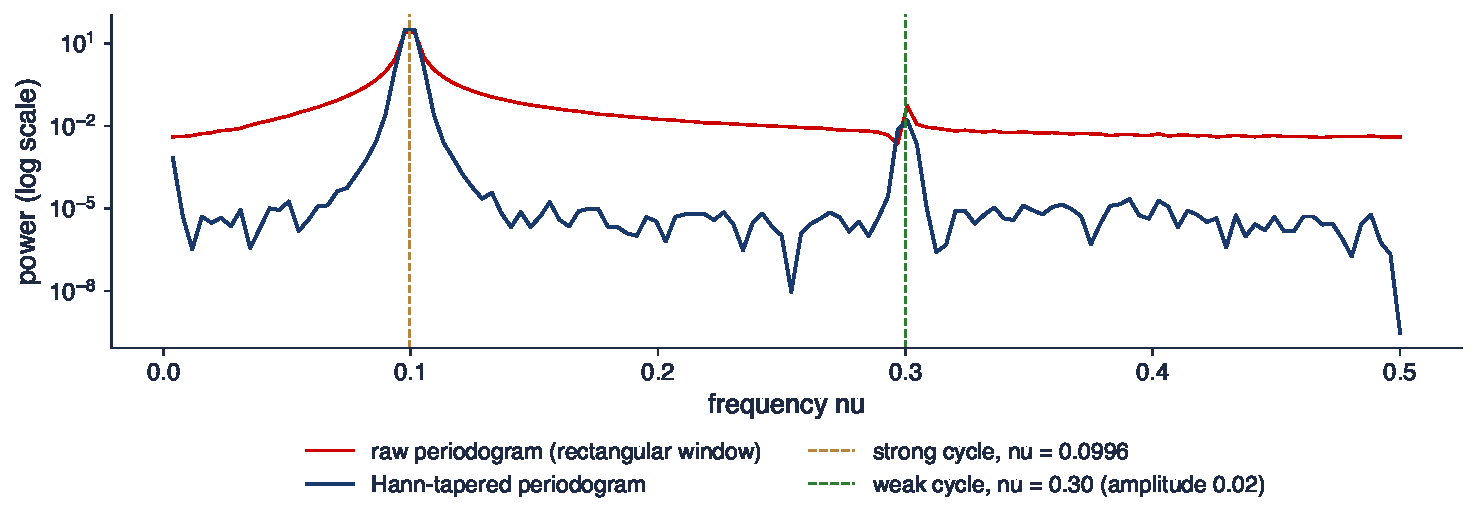
\includegraphics[width=0.97\textwidth,height=0.6\textheight,keepaspectratio]{tsa_ch12_leakage.pdf}
\end{center}
\vspace{-0.25cm}
\begin{itemize}
    \item $T = 256$: $\cos(2\pi\cdot 0{,}0996\,t)$ (între două frecvențe Fourier) plus $0{,}02\cos(2\pi\cdot 0{,}3\,t)$ și un zgomot foarte mic; scară logaritmică
\end{itemize}
\quantlet{TSA\_ch12\_leakage}{\qlurl{TSA_ch12_leakage}}
\end{frame}

\begin{frame}{Interpretarea scurgerii spectrale}
\itemsize{\small}
\begin{itemize}
    \item Periodograma brută: ciclul puternic își scurge puterea peste tot; la $\nu = 0{,}3$ ciclul slab este doar de 7{,}7 ori peste fondul scurs
    \begin{itemize}
        \item cu un zgomot real adăugat, acest vîrf slab ar fi invizibil
    \end{itemize}
    \item Fereastra Hann: fondul scade cu mai multe ordine de mărime, iar ciclul slab ajunge de 4\,230 ori peste el
    \begin{itemize}
        \item vîrful principal este puțin mai lat: atenuarea schimbă rezoluție pentru o scurgere mai mică
    \end{itemize}
    \item Scara logaritmică este esențială: pe o scară liniară ambele curbe arată ca un singur vîrf
\end{itemize}
\end{frame}

\begin{frame}{Netezirea periodogramei (1/2): estimatorul Daniell}
\itemsize{\footnotesize}
\begin{itemize}
    \item Ideea: $f$ este netedă, iar ordonatele sînt aproape independente, deci se face media a $L = 2m + 1$ ordonate vecine
    \begin{itemize}
        \item estimatorul \textbf{Daniell}: $\hat f(\nu_j) = \frac{1}{L}\sum_{k=-m}^{m} I(\nu_{j+k})$
        \item $m$: numărul de vecini de fiecare parte; $k$: parcurge valorile de la $-m$ la $m$; $\hat f$: spectrul estimat
        \item varianța este aproximativ $f^2/L$: de $L$ ori mai mică decît cea a unei singure ordonate
    \end{itemize}
    \item \textbf{Lățimea de bandă} $B = L/T$
    \begin{itemize}
        \item lățimea benzii de frecvențe peste care se face media
    \end{itemize}
    \item Compromisul deplasare--varianță: un $L$ mai mare reduce varianța, dar aplatizează vîrfurile înguste (deplasare)
    \begin{itemize}
        \item consistența cere $L \to \infty$ și $L/T \to 0$, de exemplu $L \approx \sqrt T$
    \end{itemize}
\end{itemize}
\end{frame}

\begin{frame}{Netezirea periodogramei (2/2): ferestrele de lag și metoda Welch}
\itemsize{\small}
\begin{itemize}
    \item Perspectiva echivalentă: netezirea în frecvență $=$ ponderi mai mici pentru autocovarianțele îndepărtate (ferestre de lag)
    \begin{itemize}
        \item fereastra Bartlett: $\hat f(\nu) = \sum_{|h| \le M}(1 - |h|/M)\hat\gamma(h)e^{-2\pi i\nu h}$ (\refBartlett; \refBT)
        \item $M$: lagul de trunchiere; autocovarianțele de dincolo de lagul $M$ se elimină, celelalte primesc ponderile $1 - |h|/M$, care scad liniar
        \item un $M$ mai mic înseamnă o netezire mai puternică
    \end{itemize}
    \item Metoda \textbf{Welch} (\refWelch)
    \begin{itemize}
        \item o medie a periodogramelor a $K$ segmente
        \item seria se împarte în $K$ segmente care se suprapun, se aplică fereastra pe fiecare și se face media periodogramelor
        \item \texttt{scipy.signal.welch}; lungimea segmentului fixează rezoluția
    \end{itemize}
\end{itemize}
\end{frame}

\begin{frame}{Estimări netezite ale spectrului unui AR(2)}
\itemsize{\footnotesize}
\begin{center}
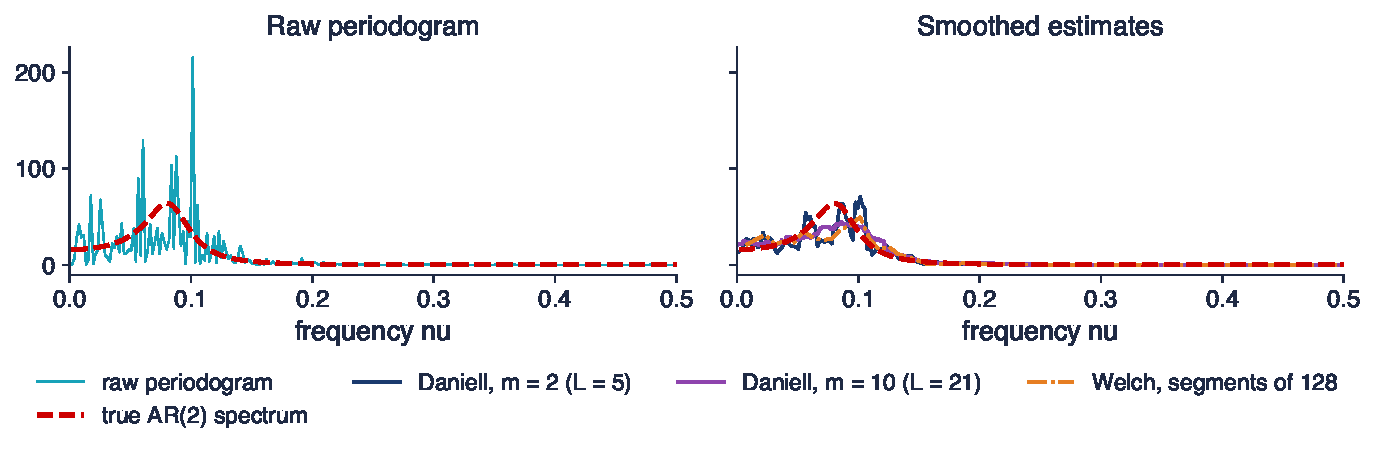
\includegraphics[width=0.97\textwidth,height=0.6\textheight,keepaspectratio]{tsa_ch12_smoothing.pdf}
\end{center}
\vspace{-0.25cm}
\begin{itemize}
    \item AR(2) simulat, $\phi = (1{,}5;\ -0{,}75)$, $T = 512$; spectrul adevărat (linie întreruptă), periodograma brută (stînga) și trei estimări netezite (dreapta)
\end{itemize}
\quantlet{TSA\_ch12\_smoothing}{\qlurl{TSA_ch12_smoothing}}
\end{frame}

\begin{frame}{Interpretarea estimărilor netezite}
\itemsize{\small}
\begin{itemize}
    \item Vîrful adevărat este la $\nu = 0{,}080$; cea mai mare ordonată brută este la $\nu = 0{,}102$: o singură ordonată zgomotoasă plasează greșit vîrful
    \begin{itemize}
        \item vîrful Daniell $m = 2$: $\nu = 0{,}102$; Daniell $m = 10$: $\nu = 0{,}086$; Welch ($K = 7$ segmente de 128): $\nu = 0{,}102$
    \end{itemize}
    \item Eroarea pătratică medie a lui $\log\hat f$: brută 1{,}86; Daniell $m = 2$: 0{,}25; $m = 10$: 0{,}09; Welch: 0{,}24
    \begin{itemize}
        \item prețul netezirii puternice: înălțimea vîrfului scade de la 64 la 44 (deplasare)
    \end{itemize}
    \item Alegeți lățimea de bandă privind mai multe valori: păstrați-o pe cea mai îngustă la care estimarea nu mai este dominată de zgomot
\end{itemize}
\end{frame}

\begin{frame}{Benzi de încredere pentru spectru}
\itemsize{\footnotesize}
\begin{itemize}
    \item Estimarea Daniell cu $L$ termeni: $\dfrac{2L\,\hat f(\nu)}{f(\nu)} \approx \chi^2_{2L}$ (grade de libertate $df = 2L$)
    \begin{itemize}
        \item intervalul de 95\%: $\left[\dfrac{df\,\hat f(\nu)}{\chi^2_{df}(0{,}975)};\ \dfrac{df\,\hat f(\nu)}{\chi^2_{df}(0{,}025)}\right]$
        \item $\chi^2_{df}(p)$: cuantila de nivel $p$ a distribuției chi-pătrat cu $df$ grade de libertate
    \end{itemize}
    \item Intervalul este un multiplu fix al lui $\hat f$: pe scară logaritmică lățimea lui este aceeași la toate frecvențele
    \begin{itemize}
        \item un vîrf este semnificativ dacă banda de la vîrf se află deasupra benzii fondului din jur
    \end{itemize}
    \item Welch cu $K$ segmente care nu se suprapun: $df \approx 2K$; suprapunerea și atenuarea modifică puțin $df$
\end{itemize}
\end{frame}

\begin{frame}{Exemplu rezolvat: o bandă de 95\% pentru $L = 5$}
\itemsize{\small}
\begin{itemize}
    \item $L = 5$ ($m = 2$), deci $df = 10$; din tabelul $\chi^2_{10}$: $\chi^2_{10}(0{,}025) = 3{,}25$ și $\chi^2_{10}(0{,}975) = 20{,}48$
    \begin{itemize}
        \item limita inferioară: $10/20{,}48 = 0{,}49$ ori $\hat f$; limita superioară: $10/3{,}25 = 3{,}08$ ori $\hat f$
    \end{itemize}
    \item Petele solare: la vîrful netezit (perioada 10{,}3 ani) $\hat f = 26\,095$
    \begin{itemize}
        \item intervalul de 95\%: [12\,740, 80\,367]: asimetric, mai lat în sus
    \end{itemize}
    \item Cu doar 5 ordonate estimarea are încă o incertitudine de un factor de 2--3; o netezire mai puternică îngustează banda, dar estompează vîrful
\end{itemize}
\end{frame}

\begin{frame}{Petele solare: spectrul netezit cu bandă de încredere}
\itemsize{\footnotesize}
\begin{center}
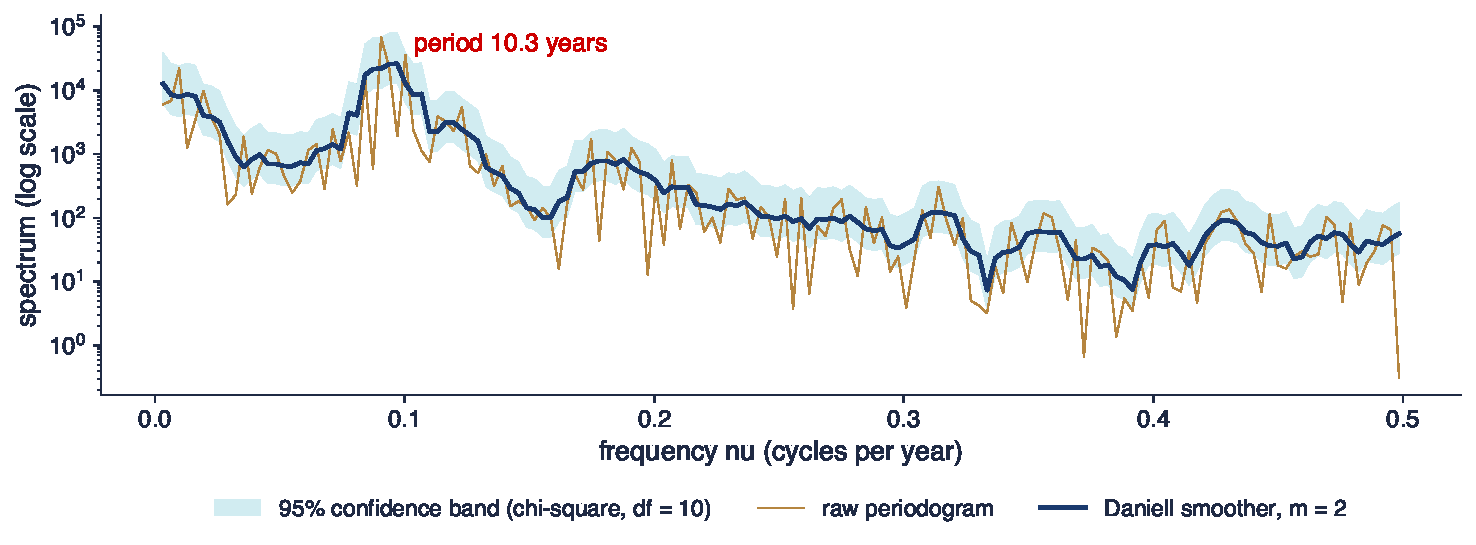
\includegraphics[width=0.97\textwidth,height=0.6\textheight,keepaspectratio]{tsa_ch12_sunspot_ci.pdf}
\end{center}
\vspace{-0.25cm}
\begin{itemize}
    \item Netezire Daniell cu $m = 2$ ($L = 5$, $df = 10$, lățimea de bandă $B = 5/309 = 0{,}016$ cicluri pe an) și banda de 95\%; scară logaritmică
\end{itemize}
\quantlet{TSA\_ch12\_sunspot\_ci}{\qlurl{TSA_ch12_sunspot_ci}}
\end{frame}

\begin{frame}{Interpretarea spectrului netezit al petelor solare}
\itemsize{\small}
\begin{itemize}
    \item Banda de la vîrf (perioada 10{,}3 ani) se află în întregime deasupra benzii fondului de la frecvențele mai înalte
    \begin{itemize}
        \item ciclul de 11 ani este o trăsătură robustă, nu un vîrf întîmplător
    \end{itemize}
    \item O a doua cocoașă, mai mică, în jurul lui $\nu \approx 0{,}18$ (aproximativ 5,5 ani) este prima \textbf{armonică}
    \begin{itemize}
        \item ciclul petelor solare nu este o sinusoidă: crește repede și scade lent, iar un ciclu nesinusoidal are putere la multiplii frecvenței lui
    \end{itemize}
    \item Puterea crește și spre $\nu = 0$: înălțimea ciclurilor se schimbă de-a lungul deceniilor și secolelor
\end{itemize}
\end{frame}

\begin{frame}{Recapitulare: estimarea spectrului}
\itemsize{\small}
\begin{itemize}
    \item Aplicați o fereastră de atenuare pentru a reduce scurgerea; reprezentați spectrele pe scară logaritmică
    \item Netezați peste $L$ ordonate (Daniell, Bartlett, Welch): varianța $\approx f^2/L$, dar vîrfurile înguste sînt aplatizate
    \item Banda de 95\%: $[df\,\hat f/\chi^2_{df}(0{,}975);\ df\,\hat f/\chi^2_{df}(0{,}025)]$, cu $df = 2L$
\end{itemize}
\end{frame}


%=============================================================================
\section{Cicluri în datele economice și energetice}
%=============================================================================

\begin{frame}{Forma spectrală tipică și ciclul economic}
\itemsize{\small}
\begin{itemize}
    \item \refGranger: spectrul majorității nivelurilor economice (PIB, prețuri) scade abrupt de la $\nu = 0$: \textbf{forma spectrală tipică}
    \begin{itemize}
        \item trendurile și rădăcinile aproape unitare pun aproape toată varianța la frecvențele cele mai joase și ascund ciclurile
        \item de aceea transformăm întîi seria într-una staționară: rate de creștere (diferențe) sau un ciclu fără trend
    \end{itemize}
    \item \textbf{Banda ciclului economic}
    \begin{itemize}
        \item fluctuații care durează între 1,5 și 8 ani, adică între 6 și 32 de trimestre (\refBK)
        \item în frecvență: $1/32 \le \nu \le 1/6$ cicluri pe trimestru
    \end{itemize}
    \item Datele: PIB-ul real al SUA (FRED GDPC1, 291 de rate de creștere trimestriale) și PIB-ul real al României (Eurostat, ajustat sezonier, 99 de rate de creștere)
    \begin{itemize}
        \item ambele pînă în T4 2019: prăbușirea și revenirea din 2020 ar domina orice periodogramă
        \item ciclul este extras și cu filtrul HP, $\lambda = 1600$ (\refHPf; \tsachlink{https://danpele.github.io/Time-Series-Analysis/RO/Cursuri/capitol10_spatiul_starilor_kalman_markov_switching.pdf}{Capitolul 10})
    \end{itemize}
\end{itemize}
\end{frame}

\begin{frame}{Creșterea PIB și ciclurile HP}
\itemsize{\footnotesize}
\begin{center}
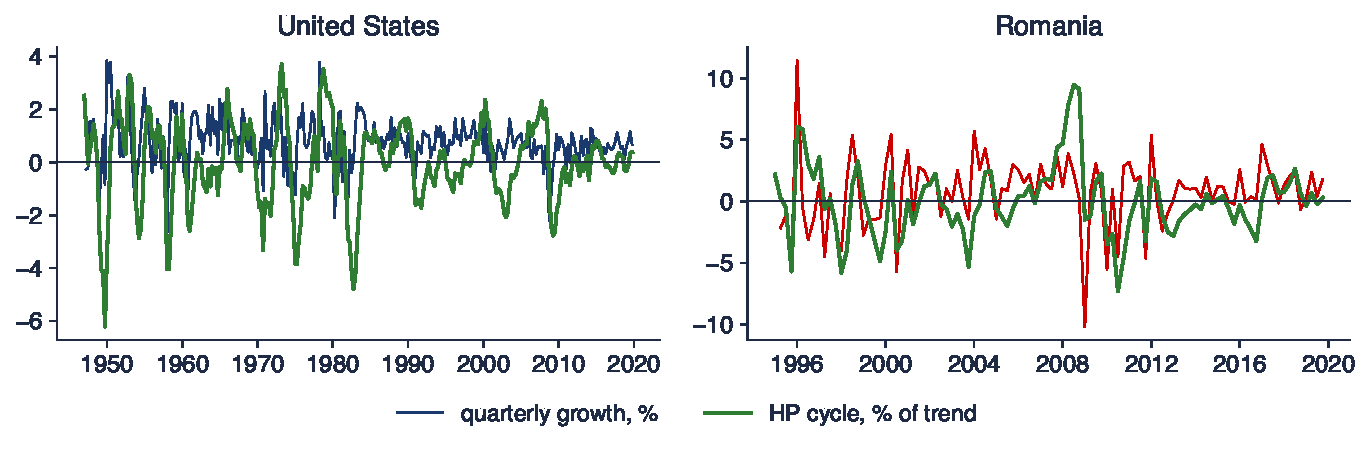
\includegraphics[width=0.97\textwidth,height=0.6\textheight,keepaspectratio]{tsa_ch12_gdp_series.pdf}
\end{center}
\vspace{-0.25cm}
\begin{itemize}
    \item Creșterea trimestrială $100\,\Delta\ln \mathrm{PIB}_t$ și ciclul HP ($100\ln\mathrm{PIB}_t$ minus trendul HP), Statele Unite 1947--2019 și România 1995--2019
\end{itemize}
\quantlet{TSA\_ch12\_gdp\_series}{\qlurl{TSA_ch12_gdp_series}}
\end{frame}

\begin{frame}{Interpretarea seriilor PIB}
\itemsize{\small}
\begin{itemize}
    \item Statele Unite: creșterea medie 0{,}78\% pe trimestru, abaterea standard 0{,}93; abaterea standard a ciclului HP 1{,}58\% din trend
    \begin{itemize}
        \item ciclul arată recesiunile ca minime adînci (1958, 1975, 1982, 2009)
    \end{itemize}
    \item România: creșterea medie 0{,}73\%, abaterea standard 2{,}85: de trei ori mai volatilă
    \begin{itemize}
        \item un singur ciclu mare de expansiune și recesiune (2004--2010) domină un eșantion de doar 25 de ani
    \end{itemize}
    \item Rata de creștere este zgomotoasă și de scurtă durată; ciclul HP este neted și persistent: spectrele lor vor fi diferite
\end{itemize}
\end{frame}

\begin{frame}{Spectrele creșterii PIB și ale ciclurilor HP}
\itemsize{\footnotesize}
\begin{center}
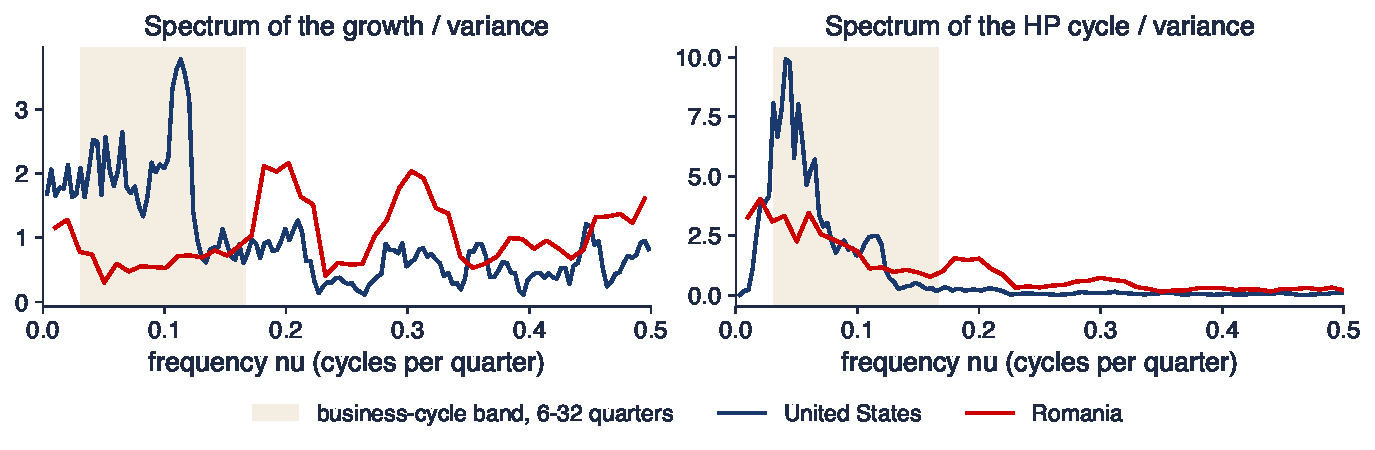
\includegraphics[width=0.97\textwidth,height=0.6\textheight,keepaspectratio]{tsa_ch12_gdp_spectra.pdf}
\end{center}
\vspace{-0.25cm}
\begin{itemize}
    \item Netezire Daniell, $m = 2$; fiecare spectru este împărțit la varianța seriei sale; hașurat: perioade între 6 și 32 de trimestre
\end{itemize}
\quantlet{TSA\_ch12\_gdp\_spectra}{\qlurl{TSA_ch12_gdp_spectra}}
\end{frame}

\begin{frame}{Interpretarea spectrelor PIB}
\itemsize{\small}
\begin{itemize}
    \item Creșterea SUA: 49\% din varianță în banda ciclului economic; vîrful netezit este la aproximativ 8{,}8 trimestre
    \begin{itemize}
        \item creșterea României: doar 16\%; cea mai mare parte a varianței este la frecvențe înalte (zgomot de la un trimestru la altul și revizuiri)
    \end{itemize}
    \item Ciclul HP al SUA: 80\% din varianță în bandă, vîrful la 24{,}3 trimestre (aproximativ 6{,}1 ani)
    \begin{itemize}
        \item ciclul HP al României: 49\% în bandă și 17\% la perioade de peste 8 ani: un singur ciclu lung într-un eșantion scurt
    \end{itemize}
    \item Atenție: filtrul HP elimină el însuși frecvențele joase și poate modela vîrful (secțiunea 7); cele 99 de observații ale României dau o bandă de încredere foarte largă
\end{itemize}
\end{frame}

\begin{frame}{Ritmul consumului de energie electrică}
\itemsize{\footnotesize}
\begin{center}
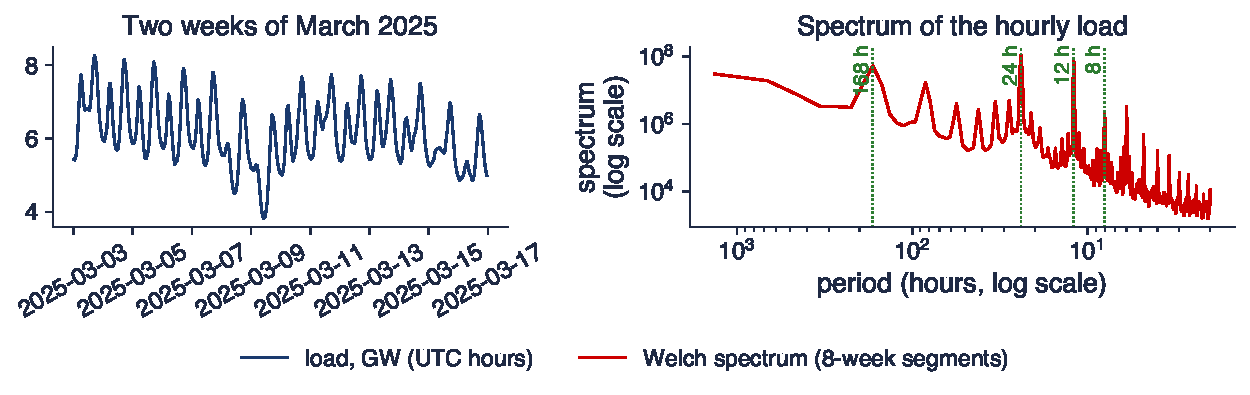
\includegraphics[width=0.97\textwidth,height=0.58\textheight,keepaspectratio]{tsa_ch12_load.pdf}
\end{center}
\vspace{-0.25cm}
\begin{itemize}
    \item Consumul orar de energie electrică al României (ENTSO-E, MW, ore UTC), 2022--2026, 39\,408 de ore, media 6\,176 MW (\tsachlink{https://danpele.github.io/Time-Series-Analysis/RO/Cursuri/capitol4_sezonalitate_prognoza.pdf}{Capitolul 4}); spectrul Welch cu segmente de 8 săptămîni
\end{itemize}
\quantlet{TSA\_ch12\_load}{\qlurl{TSA_ch12_load}}
\end{frame}

\begin{frame}{Interpretarea spectrului consumului}
\itemsize{\small}
\begin{itemize}
    \item Vîrfuri ascuțite la 24, 12 și 8 ore: ciclul zilnic și armonicele lui (vîrfurile de dimineață și de seară nu formează o sinusoidă)
    \begin{itemize}
        \item ciclul zilnic și armonicele lui explică 34\% din varianță
    \end{itemize}
    \item Un vîrf la 167{,}7 ore (o săptămînă) și armonica lui la 84{,}0 ore: zilele lucrătoare față de sfîrșitul de săptămînă
    \begin{itemize}
        \item componentele săptămînale: 16\%; perioadele mai lungi de o lună (iarna față de vară): 33\%
    \end{itemize}
    \item De aceea în \tsachlink{https://danpele.github.io/Time-Series-Analysis/RO/Cursuri/capitol4_sezonalitate_prognoza.pdf}{Capitolul 4} am modelat consumul cu termeni Fourier zilnici și săptămînali: spectrul arată ce perioade trebuie incluse
\end{itemize}
\end{frame}

\begin{frame}{Recapitulare: ciclurile din date}
\itemsize{\small}
\begin{itemize}
    \item Eliminați întîi trendurile (rate de creștere, cicluri fără trend): nivelurile au forma spectrală tipică
    \item PIB-ul SUA: un vîrf al ciclului economic de aproximativ 6{,}1 ani în ciclul HP; România: un eșantion prea scurt pentru un răspuns clar
    \item Consumul de energie electrică: cicluri zilnice și săptămînale cu armonice; spectrul alege termenii Fourier ai unui model de prognoză
\end{itemize}
\end{frame}


%=============================================================================
\section{Memoria lungă: polul de la zero}
%=============================================================================

\begin{frame}{Memoria lungă în domeniul frecvenței (1/2)}
\itemsize{\footnotesize}
\begin{itemize}
    \item \tsachlink{https://danpele.github.io/Time-Series-Analysis/RO/Cursuri/capitol8_memorie_lunga_arfima.pdf}{Capitolul 8}: o serie cu memorie lungă are autocorelații care scad ca o putere a lagului
    \begin{itemize}
        \item $\rho(h) \sim Ch^{2d-1}$: $\rho(h)$ este autocorelația la lagul $h$, $C > 0$ o constantă, iar $\sim$ înseamnă „proporțional pentru $h$ mare”
        \item $d$: parametrul de memorie; $0 < d < 1/2$ dă memorie lungă staționară; atunci $\sum_h\gamma(h) = \infty$ și $f(0) = \infty$
    \end{itemize}
    \item ARFIMA$(0,d,0)$: spectrul tinde la infinit în zero
    \begin{itemize}
        \item $f(\nu) = \sigma^2\,|2\sin(\pi\nu)|^{-2d} \approx \sigma^2(2\pi\nu)^{-2d}$ în apropierea lui $\nu = 0$: un \textbf{pol} la zero
        \item prin logaritmare: $\log f(\nu) \approx \log\sigma^2 - 2d\log(2\pi\nu)$, o dreaptă în $\log\nu$, cu panta $-2d$
    \end{itemize}
    \item Memoria scurtă (ARMA) are $f(0)$ finit: graficul log--log devine orizontal la frecvențele joase
\end{itemize}
\end{frame}

\begin{frame}{Memoria lungă în domeniul frecvenței (2/2): estimatorul GPH}
\itemsize{\small}
\begin{itemize}
    \item \refGPH: o regresie a logaritmului periodogramei pe un termen logaritmic al frecvenței
    \begin{itemize}
        \item se regresează $\log I(\nu_j)$ pe $-\log(4\sin^2(\pi\nu_j))$ pentru $j = 1, \ldots, m$; panta este $\hat d$
        \item eroarea standard $\pi/\sqrt{24m}$: scade pe măsură ce se folosesc mai multe frecvențe
    \end{itemize}
    \item Se folosesc doar cele mai joase $m = \lfloor T^{0{,}65}\rfloor$ frecvențe, unde polul domină
    \begin{itemize}
        \item un $m$ mai mare reduce eroarea standard, dar aduce efecte de memorie scurtă (deplasare)
    \end{itemize}
    \item Interpretarea
    \begin{itemize}
        \item $\hat d$ apropiat de 0: memorie scurtă; $0 < \hat d < 0{,}5$: memorie lungă staționară; $\hat d \ge 0{,}5$: nestaționaritate
    \end{itemize}
\end{itemize}
\end{frame}

\begin{frame}{Polul de la zero în datele bursiere}
\itemsize{\footnotesize}
\begin{center}
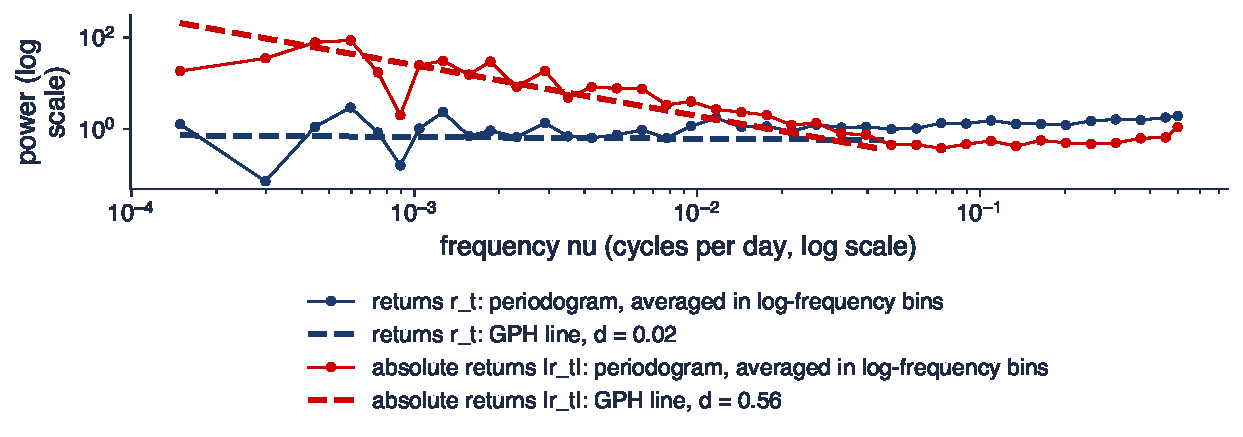
\includegraphics[width=0.97\textwidth,height=0.58\textheight,keepaspectratio]{tsa_ch12_long_memory.pdf}
\end{center}
\vspace{-0.25cm}
\begin{itemize}
    \item Randamentele logaritmice zilnice S\&P 500, 2000--2026, $T = 6\,714$ (EODHD); periodograma mediată în 40 de intervale logaritmice de frecvență; dreptele GPH pe cele mai joase $m = 307$ frecvențe (perioade de peste 22 de zile)
\end{itemize}
\quantlet{TSA\_ch12\_long\_memory}{\qlurl{TSA_ch12_long_memory}}
\end{frame}

\begin{frame}{Interpretarea periodogramei log--log}
\itemsize{\small}
\begin{itemize}
    \item Randamentele $r_t$: spectru plat la frecvențele joase, GPH $\hat d = 0{,}02$ (eroarea standard 0{,}037): nicio memorie lungă în randamente
    \begin{itemize}
        \item un spectru plat este ceea ce prevede eficiența pieței pentru randamente (\tsachlink{https://danpele.github.io/Time-Series-Analysis/RO/Cursuri/capitol1_procese_stochastice_stationaritate.pdf}{Capitolul 1})
    \end{itemize}
    \item Randamentele absolute $|r_t|$: puterea crește constant spre $\nu = 0$, panta $-2\hat d$, cu $\hat d = 0{,}56$
    \begin{itemize}
        \item memoria lungă a volatilității (\tsachlink{https://danpele.github.io/Time-Series-Analysis/RO/Cursuri/capitol8_memorie_lunga_arfima.pdf}{Capitolul 8}); un $\hat d$ apropiat de 0,5 sau peste reflectă și rupturi precum 2008 și 2020
    \end{itemize}
    \item Aceeași imagine spectrală explică de ce GPH și Whittle local (\tsachlink{https://danpele.github.io/Time-Series-Analysis/RO/Cursuri/capitol8_memorie_lunga_arfima.pdf}{Capitolul 8}) sînt estimatori din domeniul frecvenței
\end{itemize}
\end{frame}


%=============================================================================
\section{Filtre liniare}
%=============================================================================

\begin{frame}{Filtrele liniare și cîștigul lor (1/2)}
\itemsize{\small}
\begin{itemize}
    \item Un \textbf{filtru liniar} transformă o serie de intrare $x_t$ într-o serie de ieșire $y_t$ printr-o sumă ponderată a valorilor curente și trecute
    \begin{itemize}
        \item $y_t = \sum_j a_j x_{t-j}$; $a_j$: ponderile filtrului; $j$: lagul
    \end{itemize}
    \item \textbf{Răspunsul lui în frecvență} este $A(\nu) = \sum_j a_j e^{-2\pi i\nu j}$
    \begin{itemize}
        \item rezultatul de bază: $f_y(\nu) = |A(\nu)|^2 f_x(\nu)$; $f_x$, $f_y$: spectrele intrării și ieșirii
        \item $|A(\nu)|^2$ este \textbf{cîștigul pătratic}: peste 1 filtrul amplifică ciclurile de frecvență $\nu$, sub 1 le atenuează, 0 le elimină
    \end{itemize}
\end{itemize}
\end{frame}

\begin{frame}{Filtrele liniare și cîștigul lor (2/2)}
\itemsize{\small}
\begin{itemize}
    \item Prima diferență $y_t = x_t - x_{t-1}$: $|A(\nu)|^2 = |1 - e^{-2\pi i\nu}|^2 = 4\sin^2(\pi\nu)$
    \begin{itemize}
        \item zero la $\nu = 0$ (elimină trendul), 4 la $\nu = 1/2$ (amplifică zgomotul); la o perioadă de 40 de trimestre: 0{,}025; la 4 trimestre: 2
    \end{itemize}
    \item Diferența sezonieră $(1 - L^4)x_t = x_t - x_{t-4}$ (date trimestriale): cîștigul pătratic $4\sin^2(4\pi\nu)$
    \begin{itemize}
        \item zero la $\nu = 0, 1/4, 1/2$: elimină trendul și ciclurile sezoniere
    \end{itemize}
    \item Filtrul HP pentru ciclu: cîștigul pătratic $\dfrac{4\lambda(1 - \cos 2\pi\nu)^2}{1 + 4\lambda(1 - \cos 2\pi\nu)^2}$
    \begin{itemize}
        \item $\lambda$: parametrul de netezire (1600 pentru date trimestriale); un $\lambda$ mai mare mută pragul spre ciclurile mai lente
        \item aproape de 0 la frecvențele joase și aproape de 1 la cele înalte: un filtru \textbf{trece-sus}
    \end{itemize}
\end{itemize}
\end{frame}

\begin{frame}{Cîștigurile pătratice ale filtrelor uzuale}
\itemsize{\footnotesize}
\begin{center}
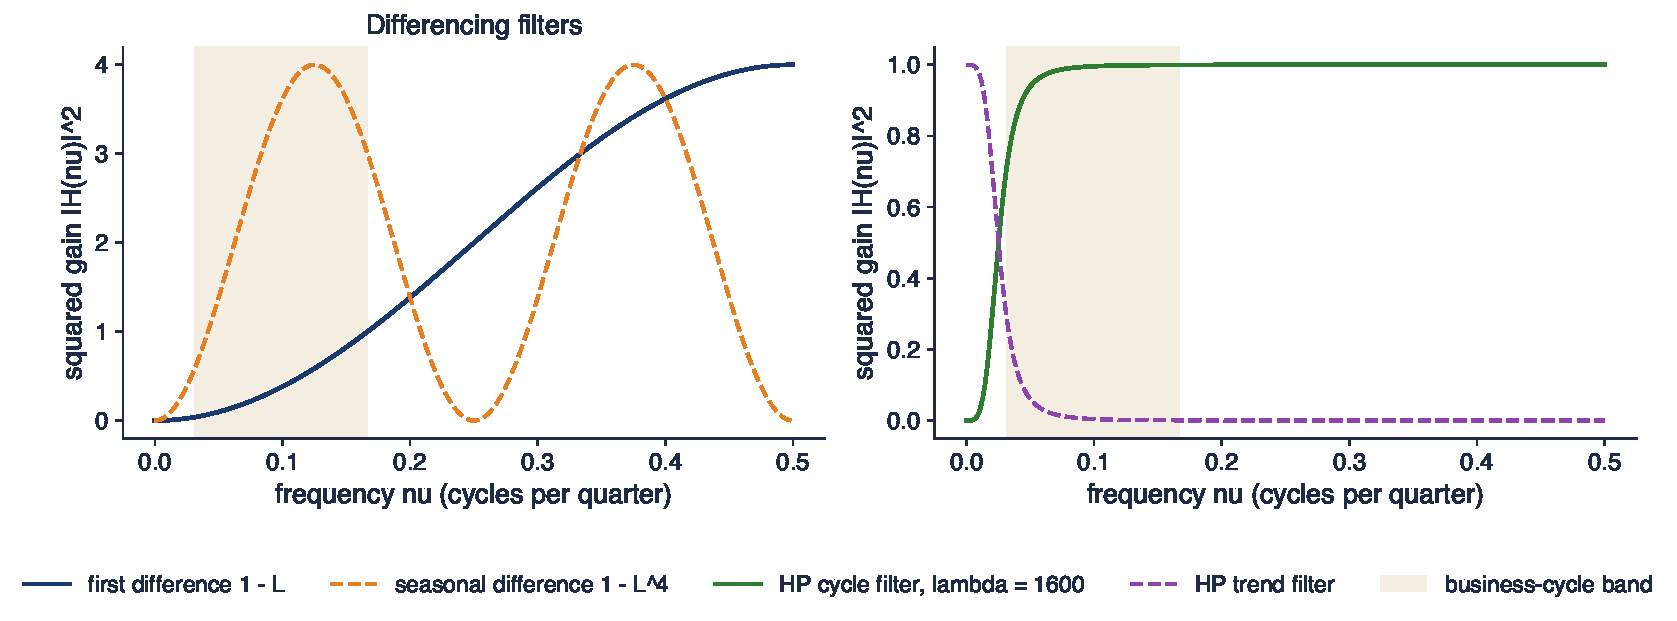
\includegraphics[width=0.97\textwidth,height=0.6\textheight,keepaspectratio]{tsa_ch12_filters.pdf}
\end{center}
\vspace{-0.25cm}
\begin{itemize}
    \item Stînga: prima diferență și diferența sezonieră ($s = 4$); dreapta: filtrele HP pentru ciclu și pentru trend, $\lambda = 1600$ (date trimestriale); hașurat: 6--32 de trimestre
\end{itemize}
\quantlet{TSA\_ch12\_filters}{\qlurl{TSA_ch12_filters}}
\end{frame}

\begin{frame}{Interpretarea cîștigurilor filtrelor}
\itemsize{\small}
\begin{itemize}
    \item Diferențierea nu este neutră: slăbește ciclurile economice și amplifică frecvențele cele mai înalte
    \begin{itemize}
        \item de aceea ratele de creștere par mai zgomotoase decît nivelurile; filtrarea unui zgomot alb poate crea chiar cicluri false (efectul Slutsky, \tsachlink{https://danpele.github.io/Time-Series-Analysis/RO/Cursuri/capitol0_introducere.pdf}{Capitolul 0})
    \end{itemize}
    \item Filtrul HP pentru ciclu: cîștig 0{,}998 la 8 trimestre, 0{,}70 la 32 de trimestre, 0{,}49 la 40 de trimestre; jumătate din putere la aproximativ 40 de trimestre
    \begin{itemize}
        \item păstrează tot ce este mai rapid de 10 ani, inclusiv zgomotul: nu este un filtru trece-bandă (\refBK)
    \end{itemize}
    \item Aplicat unui mers aleator, filtrul HP produce un ciclu cu un vîrf care provine din filtru, nu din date (\refHamHP)
\end{itemize}
\end{frame}


%=============================================================================
\section{Două serii: coerență și fază}
%=============================================================================

\begin{frame}{Spectrul încrucișat, coerența și faza}
\itemsize{\footnotesize}
\begin{itemize}
    \item Pentru două serii staționare cu covarianțele încrucișate $\gamma_{xy}(h) = \mathrm{Cov}(x_{t+h}, y_t)$:
    \begin{itemize}
        \item \textbf{spectrul încrucișat} $f_{xy}(\nu) = \sum_h\gamma_{xy}(h)e^{-2\pi i\nu h}$, un număr complex la fiecare frecvență
        \item $f_x$, $f_y$: spectrele lui $x$ și $y$, luate separat
    \end{itemize}
    \item \textbf{Coerența pătratică}
    \begin{itemize}
        \item $\rho^2_{xy}(\nu) = \dfrac{|f_{xy}(\nu)|^2}{f_x(\nu)f_y(\nu)} \in [0, 1]$
        \item un pătrat al corelației, frecvență cu frecvență: cît de bine se mișcă împreună ciclurile lui $x$ și $y$ la frecvența $\nu$
    \end{itemize}
    \item \textbf{Faza} $\varphi(\nu) = \arg f_{xy}(\nu)$
    \begin{itemize}
        \item defazajul dintre cele două cicluri, în radiani
        \item $\arg$: unghiul unui număr complex în plan (argumentul lui)
        \item un lag de $k$ perioade dă o fază liniară în frecvență: $\varphi(\nu) = \pm 2\pi\nu k$; deci lagul este $|\varphi|/(2\pi\nu)$
    \end{itemize}
    \item Estimarea: netezim periodograma încrucișată la fel ca periodograma; coerența brută este întotdeauna 1, deci netezirea este obligatorie
\end{itemize}
\end{frame}

\begin{frame}{Producția industrială și șomajul}
\itemsize{\footnotesize}
\begin{center}
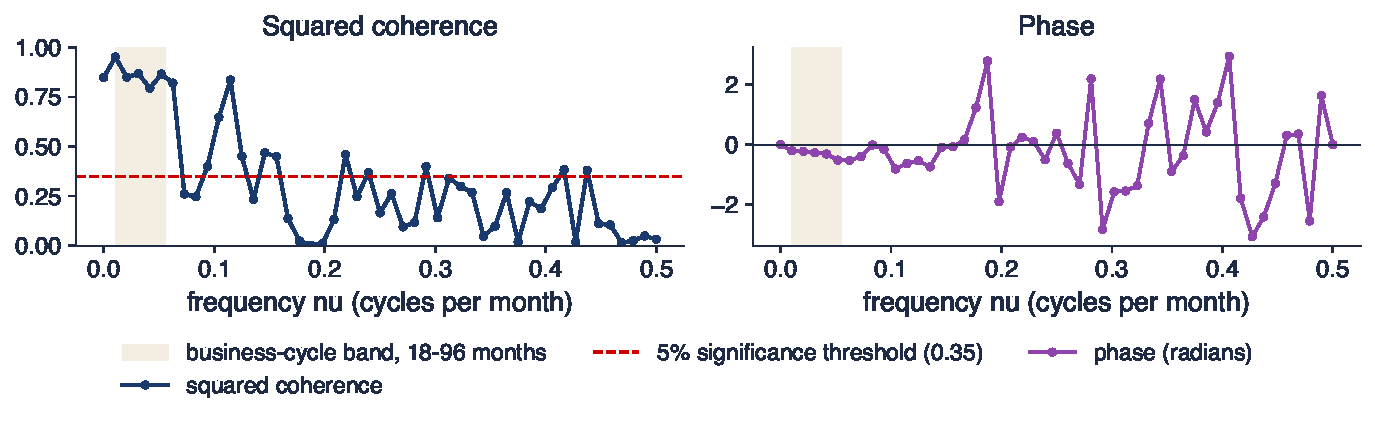
\includegraphics[width=0.97\textwidth,height=0.56\textheight,keepaspectratio]{tsa_ch12_coherence.pdf}
\end{center}
\vspace{-0.25cm}
\begin{itemize}
    \item Date lunare din SUA, 1948--2019 (FRED INDPRO, UNRATE), $T = 863$: $x_t = 100\,\Delta\ln \mathrm{IP}_t$ și $y_t = -\Delta u_t$ (scăderea ratei șomajului); Welch cu $K = 8$ segmente de 96 de luni
\end{itemize}
\quantlet{TSA\_ch12\_coherence}{\qlurl{TSA_ch12_coherence}}
\end{frame}

\begin{frame}{Interpretarea coerenței și fazei}
\itemsize{\small}
\begin{itemize}
    \item În banda ciclului economic (18--96 de luni) coerența pătratică are media 0{,}87 (maximum 0{,}95), mult peste pragul de 5\%, 0{,}35
    \begin{itemize}
        \item la frecvențele mai rapide de 6 luni media este doar 0{,}17: zgomotul lunar al celor două serii nu este legat
        \item corelația obișnuită, 0{,}49, amestecă legătura puternică a ciclurilor cu legătura slabă a zgomotului
    \end{itemize}
    \item Faza la ciclul de 48 de luni: -0{,}23 radiani, un lag de aproximativ 1{,}7 luni
    \begin{itemize}
        \item scăderea șomajului urmează revenirea producției cu o mică întîrziere (legea lui Okun, cu un lag)
    \end{itemize}
    \item Acolo unde coerența este mică, faza nu are sens: citiți faza doar în benzile cu coerență semnificativă
\end{itemize}
\end{frame}


%=============================================================================
\section{O trimitere: wavelets}
%=============================================================================

\begin{frame}{Wavelets: frecvența care se schimbă în timp}
\itemsize{\small}
\begin{itemize}
    \item Spectrul presupune staționaritate: aceleași cicluri la orice dată
    \begin{itemize}
        \item \textbf{transformata Fourier pe ferestre scurte} (STFT) calculează spectre în ferestre mobile de lungime fixă
    \end{itemize}
    \item Un \textbf{wavelet} este un pachet scurt de unde; \textbf{transformata wavelet continuă} (CWT) îl întinde la fiecare perioadă și îl glisează de-a lungul seriei
    \begin{itemize}
        \item rezultatul, \textbf{scalograma}, arată puterea la fiecare perioadă și la fiecare dată (\refTC)
        \item ferestre scurte pentru ciclurile rapide, ferestre lungi pentru ciclurile lente: rezoluție bună la toate scările
    \end{itemize}
    \item Dincolo de acest curs; o temă naturală de proiect (Python: \texttt{pywt} sau codul Morlet al acestui capitol)
\end{itemize}
\end{frame}

\begin{frame}{Puterea wavelet a petelor solare}
\itemsize{\footnotesize}
\begin{center}
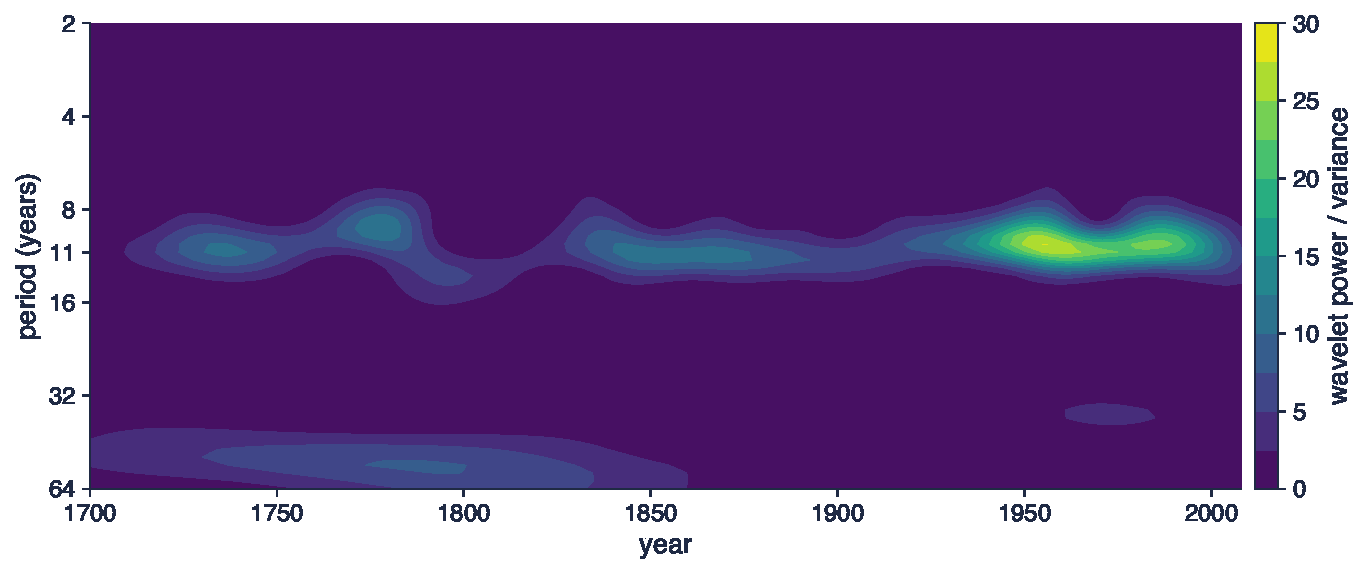
\includegraphics[width=0.97\textwidth,height=0.56\textheight,keepaspectratio]{tsa_ch12_wavelet.pdf}
\end{center}
\vspace{-0.25cm}
\begin{itemize}
    \item Puterea wavelet Morlet a numerelor anuale standardizate de pete solare, 1700--2008, perioade între 2 și 64 de ani; culorile deschise indică putere mare
\end{itemize}
\quantlet{TSA\_ch12\_wavelet}{\qlurl{TSA_ch12_wavelet}}
\end{frame}

\begin{frame}{Interpretarea scalogramei}
\itemsize{\small}
\begin{itemize}
    \item Banda de 11 ani este prezentă tot timpul, dar intensitatea ei se schimbă
    \begin{itemize}
        \item puterea medie în banda de 8--14 ani: 2{,}0 în 1795--1830 (minimul Dalton, cu cicluri slabe), față de 5{,}7 pe întregul eșantion; maximul este în jurul anului 1956
    \end{itemize}
    \item Periodograma a mediat aceste schimbări într-un singur vîrf; scalograma arată cînd ciclul a fost puternic sau slab
    \item Marginile graficului sînt mai puțin sigure (wavelet-ul rămîne fără date): această regiune se numește conul de influență
\end{itemize}
\end{frame}

\begin{frame}{Recapitulare: memoria lungă, filtre, două serii, wavelets}
\itemsize{\small}
\begin{itemize}
    \item Memoria lungă este un pol la $\nu = 0$: panta $-2d$ pe un grafic log--log (GPH)
    \item Un filtru înmulțește spectrul cu cîștigul lui pătratic: diferențierea și filtrul HP remodelează ciclurile
    \item Coerența este o corelație pe frecvențe; faza arată avansul sau lagul unei serii față de cealaltă
    \item Wavelets arată cum se schimbă ciclurile în timp
\end{itemize}
\end{frame}


%=============================================================================
\section{Contribuția posibilă a AI}
%=============================================================================

\begin{frame}{Contribuția posibilă a AI}
\itemsize{\small}
\begin{itemize}
    \item \textbf{Cod}
    \begin{itemize}
        \item o primă versiune a unei periodograme, a unei neteziri Daniell, a unei estimări Welch sau a unui grafic al coerenței
    \end{itemize}
    \item \textbf{Explicații}
    \begin{itemize}
        \item o a doua explicație a scurgerii spectrale, a fenomenului de aliasing sau a compromisului deplasare--varianță al lățimii de bandă
    \end{itemize}
    \item \textbf{Explorare}
    \begin{itemize}
        \item spectrele multor serii deodată (consumul mai multor țări, PIB-ul tuturor statelor UE) și o primă interpretare a vîrfurilor
    \end{itemize}
    \item Exemplu de prompt
    \begin{itemize}
        \item \aiprompt{Write Python code that reads hourly electricity load, removes the mean, computes the periodogram with a Hann taper and a Welch estimate with 8-week segments, plots both on a log-log scale against the period in hours, and marks 24, 12 and 168 hours.}
    \end{itemize}
\end{itemize}
\end{frame}

\begin{frame}{Verificări necesare}
\itemsize{\small}
\begin{itemize}
    \item Unitățile: frecvența în cicluri pe observație sau în radiani; \texttt{scipy.signal.welch} întoarce o densitate unilaterală (dublul lui $f$)
    \item Perioada: $1/\nu$ în observații; transformați-o singuri în ani, trimestre sau ore
    \item Parseval: ordonatele trebuie să se adune la $T$ înmulțit cu varianța; testați codul pe un cosinus cu frecvență cunoscută
    \item Un vîrf este un ciclu doar cu un test sau cu o bandă de încredere; o periodogramă brută are întotdeauna vîrfuri înalte
    \item Trendurile, rupturile și filtrele creează putere la frecvențele joase și vîrfuri false: verificați întîi datele și transformarea
    \item Fiecare referință citată: trebuie să existe; verificați DOI-ul
\end{itemize}
\end{frame}


%=============================================================================
\section{Rezumat}
%=============================================================================

\begin{frame}{Idei de reținut}
\itemsize{\small}
\begin{itemize}
    \item Spectrul împarte varianța unei serii staționare pe frecvențe; conține aceeași informație ca ACF
    \item Interpretați forma lui: plat (zgomot alb), descrescător (persistență), cu vîrfuri (cicluri), cu pol la zero (memorie lungă)
    \item Periodograma brută este nedeplasată, dar neconsistentă: aplicați atenuarea, netezirea și benzile de încredere
    \item Cicluri reale: 11 ani la petele solare, 4--8 ani în PIB, 24 de ore și o săptămînă în consumul de energie electrică
    \item Filtrele remodelează spectrele; coerența și faza leagă ciclurile a două serii
\end{itemize}
\end{frame}

\begin{frame}{Formule de reținut}
\itemsize{\small}
{\renewcommand{\arraystretch}{1.35}\begin{center}
\scriptsize
\begin{tabular}{ll}
\toprule
\textbf{Mărimea} & \textbf{Formula} \\
\midrule
Densitatea spectrală & $f(\nu) = \sum_h\gamma(h)e^{-2\pi i\nu h}$, \quad $\gamma(0) = \int_{-1/2}^{1/2} f(\nu)\,d\nu$ \\
AR(1), MA(1) & $\sigma^2/(1 - 2\phi\cos 2\pi\nu + \phi^2)$, \quad $\sigma^2(1 + 2\theta\cos 2\pi\nu + \theta^2)$ \\
ARMA & $\sigma^2|\theta(e^{-2\pi i\nu})|^2/|\phi(e^{-2\pi i\nu})|^2$ \\
Periodograma & $I(\nu_j) = |T^{-1/2}\sum_t x_t e^{-2\pi i\nu_j t}|^2$, \quad $\nu_j = j/T$, \quad $2I/f \approx \chi^2_2$ \\
Daniell & $\hat f(\nu_j) = \frac1L\sum_{|k| \le m} I(\nu_{j+k})$, \quad $L = 2m + 1$, \quad $B = L/T$ \\
Banda de 95\% & $[2L\hat f/\chi^2_{2L}(0{,}975),\ 2L\hat f/\chi^2_{2L}(0{,}025)]$ \\
Filtru liniar & $f_y(\nu) = |A(\nu)|^2 f_x(\nu)$, \quad $|1 - e^{-2\pi i\nu}|^2 = 4\sin^2(\pi\nu)$ \\
Coerența, faza & $\rho^2_{xy} = |f_{xy}|^2/(f_x f_y)$, \quad $\varphi = \arg f_{xy}$, \quad lagul $= |\varphi|/(2\pi\nu)$ \\
\bottomrule
\end{tabular}
\end{center}
}
\end{frame}

\begin{frame}{Autoevaluare (1/2)}
\itemsize{\footnotesize}
\begin{itemize}
    \item \textbf{Întrebare}: niște date săptămînale au un vîrf la $\nu = 0{,}0192$. Care este perioada?
    \begin{itemize}
        \item \textbf{Răspuns}: $1/0{,}0192 \approx 52$ de săptămîni: un ciclu anual
    \end{itemize}
    \item \textbf{Întrebare}: cît sînt $f(0)$ și $f(1/2)$ pentru un AR(1) cu $\phi = -0{,}5$, $\sigma^2 = 1$?
    \begin{itemize}
        \item \textbf{Răspuns}: $f(0) = 1/1{,}5^2 = 0{,}44$ și $f(1/2) = 1/0{,}5^2 = 4$: puterea este la frecvențele înalte
    \end{itemize}
    \item \textbf{Întrebare}: de ce un eșantion mai lung nu face periodograma brută mai precisă?
    \begin{itemize}
        \item \textbf{Răspuns}: fiecare ordonată are în continuare varianța aproximativ $f^2$; mai multe date adaugă doar ordonate; precizia cere o mediere
    \end{itemize}
    \item \textbf{Întrebare}: pentru $L = 5$, cît de largă este banda de 95\% în raport cu $\hat f$?
    \begin{itemize}
        \item \textbf{Răspuns}: de la 0{,}49 la 3{,}08 ori $\hat f$ ($df = 10$)
    \end{itemize}
\end{itemize}
\end{frame}

\begin{frame}{Autoevaluare (2/2)}
\itemsize{\footnotesize}
\begin{itemize}
    \item \textbf{Întrebare}: o serie lunară observată doar o dată la două luni are un ciclu de 3 luni. Unde apare acesta?
    \begin{itemize}
        \item \textbf{Răspuns}: $\nu = 2/3$ cicluri la două luni este peste $1/2$; se pliază la $1/3$: un ciclu fals de 3 observații, adică 6 luni
    \end{itemize}
    \item \textbf{Întrebare}: ce efect are prima diferență asupra unui ciclu de 40 de trimestre?
    \begin{itemize}
        \item \textbf{Răspuns}: îi înmulțește puterea cu $4\sin^2(\pi/40) = 0{,}025$: ciclul aproape dispare
    \end{itemize}
    \item \textbf{Întrebare}: periodograma log--log a unei serii are panta $-0{,}6$ în apropierea lui zero. Cît este $d$?
    \begin{itemize}
        \item \textbf{Răspuns}: panta $= -2d$, deci $d = 0{,}3$: memorie lungă staționară (\tsachlink{https://danpele.github.io/Time-Series-Analysis/RO/Cursuri/capitol8_memorie_lunga_arfima.pdf}{Capitolul 8})
    \end{itemize}
    \item \textbf{Întrebare}: coerența pătratică a două serii este 0,9 la ciclurile de 5 ani și 0,1 la ciclurile lunare. Ce înseamnă aceasta?
    \begin{itemize}
        \item \textbf{Răspuns}: ciclurile lor economice se mișcă împreună; zgomotul lor pe termen scurt nu
    \end{itemize}
    \item Urmează: \tsachlink{https://danpele.github.io/Time-Series-Analysis/RO/Cursuri/capitol13_bule_lppl.pdf}{Capitolul 13}, bule speculative și modele LPPL
\end{itemize}
\end{frame}


%=============================================================================
\section{Bibliografie}
%=============================================================================

\begin{frame}{Bibliografie (1/2)}
\itemsize{\tiny}
\begin{itemize}
    \item Bartlett, M. S. (1950). Periodogram analysis and continuous spectra. \textit{Biometrika}, 37(1--2), 1--16. \href{https://doi.org/10.1093/biomet/37.1-2.1}{doi:10.1093/biomet/37.1-2.1}
    \item Baxter, M., \& King, R. G. (1999). Measuring business cycles: Approximate band-pass filters for economic time series. \textit{Review of Economics and Statistics}, 81(4), 575--593. \href{https://doi.org/10.1162/003465399558454}{doi:10.1162/003465399558454}
    \item Blackman, R. B., \& Tukey, J. W. (1958). The measurement of power spectra from the point of view of communications engineering, Part I. \textit{Bell System Technical Journal}, 37(1), 185--282. \href{https://doi.org/10.1002/j.1538-7305.1958.tb03874.x}{doi:10.1002/j.1538-7305.1958.tb03874.x}
    \item Brockwell, P. J., \& Davis, R. A. (1991). \textit{Time Series: Theory and Methods} (2nd ed.). Springer. \href{https://doi.org/10.1007/978-1-4419-0320-4}{doi:10.1007/978-1-4419-0320-4}
    \item Cooley, J. W., \& Tukey, J. W. (1965). An algorithm for the machine calculation of complex Fourier series. \textit{Mathematics of Computation}, 19(90), 297--301. \href{https://doi.org/10.1090/S0025-5718-1965-0178586-1}{doi:10.1090/S0025-5718-1965-0178586-1}
    \item Fisher, R. A. (1929). Tests of significance in harmonic analysis. \textit{Proceedings of the Royal Society of London, Series A}, 125(796), 54--59. \href{https://doi.org/10.1098/rspa.1929.0151}{doi:10.1098/rspa.1929.0151}
    \item Geweke, J., \& Porter-Hudak, S. (1983). The estimation and application of long memory time series models. \textit{Journal of Time Series Analysis}, 4(4), 221--238. \href{https://doi.org/10.1111/j.1467-9892.1983.tb00371.x}{doi:10.1111/j.1467-9892.1983.tb00371.x}
    \item Granger, C. W. J. (1966). The typical spectral shape of an economic variable. \textit{Econometrica}, 34(1), 150--161. \href{https://doi.org/10.2307/1909859}{doi:10.2307/1909859}
    \item Hamilton, J. D. (1994). \textit{Time Series Analysis}. Princeton University Press. \href{https://doi.org/10.1515/9780691218632}{doi:10.1515/9780691218632}
\end{itemize}
\end{frame}

\begin{frame}{Bibliografie (2/2)}
\itemsize{\tiny}
\begin{itemize}
    \item Hamilton, J. D. (2018). Why you should never use the Hodrick--Prescott filter. \textit{Review of Economics and Statistics}, 100(5), 831--843. \href{https://doi.org/10.1162/rest_a_00706}{doi:10.1162/rest\_a\_00706}
    \item Hodrick, R. J., \& Prescott, E. C. (1997). Postwar U.S. business cycles: An empirical investigation. \textit{Journal of Money, Credit and Banking}, 29(1), 1--16. \href{https://doi.org/10.2307/2953682}{doi:10.2307/2953682}
    \item Huang, C., \& Petukhina, A. (2022). \textit{Applied Time Series Analysis and Forecasting with Python}. Springer. \href{https://doi.org/10.1007/978-3-031-13584-2}{doi:10.1007/978-3-031-13584-2}
    \item Schuster, A. (1898). On the investigation of hidden periodicities with application to a supposed 26 day period of meteorological phenomena. \textit{Terrestrial Magnetism}, 3(1), 13--41. \href{https://doi.org/10.1029/TM003i001p00013}{doi:10.1029/TM003i001p00013}
    \item Shumway, R. H., \& Stoffer, D. S. (2017). \textit{Time Series Analysis and Its Applications: With R Examples} (4th ed.). Springer. \href{https://doi.org/10.1007/978-3-319-52452-8}{doi:10.1007/978-3-319-52452-8}
    \item Torrence, C., \& Compo, G. P. (1998). A practical guide to wavelet analysis. \textit{Bulletin of the American Meteorological Society}, 79(1), 61--78. \href{https://doi.org/10.1175/1520-0477(1998)079<0061:APGTWA>2.0.CO;2}{doi:10.1175/1520-0477(1998)079<0061:APGTWA>2.0.CO;2}
    \item Welch, P. D. (1967). The use of fast Fourier transform for the estimation of power spectra: A method based on time averaging over short, modified periodograms. \textit{IEEE Transactions on Audio and Electroacoustics}, 15(2), 70--73. \href{https://doi.org/10.1109/TAU.1967.1161901}{doi:10.1109/TAU.1967.1161901}
    \item Yule, G. U. (1927). On a method of investigating periodicities in disturbed series, with special reference to Wolfer's sunspot numbers. \textit{Philosophical Transactions of the Royal Society of London, Series A}, 226, 267--298. \href{https://doi.org/10.1098/rsta.1927.0007}{doi:10.1098/rsta.1927.0007}
\end{itemize}
\end{frame}

\end{document}
